% ------------------------------------------------------------------------
% ------------------------------------------------------------------------
% Modelo UFSC para Trabalhos Academicos (tese de doutorado, dissertação de
% mestrado) utilizando a classe abntex2
%
% Autor: Alisson Lopes Furlani
% 	Modificações:
%	- 27/08/2019: Alisson L. Furlani, add pacote 'glossaries' para listas
%   - 06/11/2019: Luiz-Rafael Santos, modifica para Trabalho de Conclusão de Curso
% ------------------------------------------------------------------------
% ------------------------------------------------------------------------

\documentclass[
	% -- opções da classe memoir --
	12pt,				% tamanho da fonte
	%openright,			% capítulos começam em pág ímpar (insere página vazia caso preciso)
	oneside,			% para impressão no anverso. Oposto a twoside
	a4paper,			% tamanho do papel. 
	% -- opções da classe abntex2 --
	chapter=TITLE,		% títulos de capítulos convertidos em letras maiúsculas
	section=TITLE,		% títulos de seções convertidos em letras maiúsculas
	%subsection=TITLE,	% títulos de subseções convertidos em letras maiúsculas
	%subsubsection=TITLE,% títulos de subsubseções convertidos em letras maiúsculas
	% -- opções do pacote babel --
	english,			% idioma adicional para hifenização
	%french,				% idioma adicional para hifenização
	%spanish,			% idioma adicional para hifenização
	brazil				% o último idioma é o principal do documento
	]{abntex2}

\usepackage{setup/ufscthesisA4-alf}

% ---
% Filtering and Mapping Bibliographies
% ---
% Pacotes de citações
% ---
\usepackage{csquotes}
\usepackage[backend = biber, style = abnt]{biblatex}
% FIXME Se desejar estilo numérico de citações,  comente a linha acima e descomente a linha a seguir.
% \usepackage[backend = biber, style = numeric-comp]{biblatex}
\usepackage{glossaries-extra}
\usepackage{hyperref} 
\usepackage{color}


%%%%%%%%%%%%%%%%%%%%%%%%%%%%%%%%%%%%%%%%%%%%%%%%%%%%%%%%%%%%%%%%%%%%
%%% Usado para destacar problemas de escrita e considerações     %%%
%%%%%%%%%%%%%%%%%%%%%%%%%%%%%%%%%%%%%%%%%%%%%%%%%%%%%%%%%%%%%%%%%%%%
%\newcommand{\revisorA}[1]{\textcolor{blue}{#1}} 
%\newcommand{\revisorB}[1]{\textcolor{red}{#1}} 
\newcommand{\attention}[1]{{\color{red}\textbf{#1}}}
\newcommand{\propFileto}[1]{\textcolor{blue}{#1}} 
\newcommand{\propGustavo}[1]{\textcolor{magenta}{#1}}


\setlength\bibitemsep{\baselineskip}
\DeclareFieldFormat{url}{Disponível~em:\addspace\url{#1}}
\NewBibliographyString{sineloco}
\NewBibliographyString{sinenomine}
\DefineBibliographyStrings{brazil}{%
	sineloco     = {\mkbibemph{S\adddot l\adddot}},
	sinenomine   = {\mkbibemph{s\adddot n\adddot}},
	andothers    = {\mkbibemph{et\addabbrvspace al\adddot}},
	in			 = {\mkbibemph{In:}}
}

\addbibresource{aftertext/references.bib} % Seus arquivos de referências

% ---
\DeclareSourcemap{
	\maps[datatype=bibtex]{
		% remove fields that are always useless
		\map{
			\step[fieldset=abstract, null]
			\step[fieldset=pagetotal, null]
		}
		% remove URLs for types that are primarily printed
%		\map{
%			\pernottype{software}
%			\pernottype{online}
%			\pernottype{report}
%			\pernottype{techreport}
%			\pernottype{standard}
%			\pernottype{manual}
%			\pernottype{misc}
%			\step[fieldset=url, null]
%			\step[fieldset=urldate, null]
%		}
		\map{
			\pertype{inproceedings}
			% remove mostly redundant conference information
			\step[fieldset=venue, null]
			\step[fieldset=eventdate, null]
			\step[fieldset=eventtitle, null]
			% do not show ISBN for proceedings
			\step[fieldset=isbn, null]
			% Citavi bug
			\step[fieldset=volume, null]
		}
	}
}
% ---

% ---
% Informações de dados para CAPA e FOLHA DE ROSTO
% ---
% FIXME Substituir 'Nome completo do autor' pelo seu nome.
\autor{Gustavo Fukushima de Salles}
% FIXME Substituir 'Título do trabalho' pelo título da trabalho.
\titulo{Extração, transformação e carga de dados sobre compras da Prefeitura de Florianópolis usando Airflow}
% FIXME Substituir 'Subtítulo (se houver)' pelo subtítulo da trabalho.  
% Caso não tenha substítulo, comente a linha a seguir.
% \subtitulo{Subtítulo (se houver)}
% FIXME Substituir 'XXXXXX' pelo nome do seu
% orientador.
\orientador{Prof. Renato Fileto, Dr.}
% FIXME Se for orientado por uma mulher, comente a linha acima e descomente a linha a seguir.
% \orientador[Orientadora]{Nome da orientadora, Dra.}
% FIXME Substituir 'XXXXXX' pelo nome do seu
% coorientador. Caso não tenha coorientador, comente a linha a seguir.
% \coorientador{Prof. XXXXXX, Dr.}
% FIXME Se for coorientado por uma mulher, comente a linha acima e descomente a linha a seguir.
% \coorientador[Coorientadora]{XXXXXX, Dra.}
% FIXME Substituir 'XXXXXX' pelo nome do Coordenador do 
% programa/curso.
\coordenador{Prof. XXXXXX, Dr.}
% FIXME Se for coordenadora mulher, comente a linha acima e descomente a linha a seguir.
% \coordenador[Coordenadora]{Nome da Coordenadora, Dra.}
% FIXME Substituir '[ano da entrega]' pelo ano (ano) em que seu trabalho foi defendido.
\ano{2025}
% FIXME Substituir '[dia] de [mês] de [ano]' pela data em que ocorreu sua defesa.
\data{[dia] de [mês] de [ano]}
% FIXME Substituir '[Cidade da defesa]' pela cidade em que ocorreu sua defesa.
\local{Florianópolis}
\instituicaosigla{UFSC}
\instituicao{Universidade Federal de Santa Catarina}
% FIXME Substituir 'Dissertação/Tese' pelo tipo de trabalho (Tese, Dissertação). 
\tipotrabalho{Trabalho de Conclusão de Curso}
% FIXME Substituir '[licenciado/bacharel] em [nome do título obtido]' pela grau adequado.
\formacao{bacharel em Ciências da Computação}
% FIXME Substituir '[licenciado/bacharel]' pelo nivel adequado.
\nivel{bacharel}
% FIXME Substituir 'Curso de Graduação em [XXXXXXXX]' pela curso adequado.
\programa{Curso de Graduação em Ciências da Computação}
% FIXME Substituir 'Campus XXXXXX ou Centro de XXXXXX' pelo campus ou centro adequado.
\centro{Centro Tecnológico}
\preambulo
{%
\imprimirtipotrabalho~do~\imprimirprograma~do~\imprimircentro~da~\imprimirinstituicao~para~a~obtenção~do~título~de~\imprimirformacao.
}
% ---

% ---
% Configurações de aparência do PDF final
% ---
% alterando o aspecto da cor azul
\definecolor{blue}{RGB}{41,5,195}
% informações do PDF
\makeatletter
\hypersetup{
     	%pagebackref=true,
		pdftitle={\@title}, 
		pdfauthor={\@author},
    	pdfsubject={\imprimirpreambulo},
	    pdfcreator={LaTeX with abnTeX2},
		pdfkeywords={ufsc, latex, abntex2}, 
		colorlinks=true,       		% false: boxed links; true: colored links
    	linkcolor=black,%blue,          	% color of internal links
    	citecolor=black,%blue,        		% color of links to bibliography
    	filecolor=black,%magenta,      		% color of file links
		urlcolor=black,%blue,
		bookmarksdepth=4
}
\makeatother
% ---

% ---
% compila a lista de abreviaturas e siglas e a lista de símbolos
% ---

% Declaração das siglas
\siglalista{API}{\textit{Application Programming Interface}}
\siglalista{CSV}{\textit{Comma-separated Values}}
\siglalista{DAG}{\textit{Directed Acyclic Graph}}
\siglalista{ETL}{\textit{Extract, Transform, Load}}
\siglalista{HTTP}{\textit{Hypertext Transfer Protocol}}
\siglalista{JSON}{\textit{JavaScript Object Notation}}
\siglalista{MPSC}{Ministério Público de Santa Catarina}
\siglalista{PDF}{\textit{Portable Document Format}}
\siglalista{PMF}{Prefeitura Municipal de Florianópolis}
\siglalista{REST}{\textit{Representational State Transfer}}
\siglalista{URL}{\textit{Uniform Resource Locator}}
\siglalista{XML}{\textit{Extensible Markup Language}}

% Declaração dos simbolos

% compila a lista de abreviaturas e siglas e a lista de símbolos
\makenoidxglossaries 

% ---

% ---
% compila o indice
% ---
\makeindex
% ---

% ----
% Início do documento
% ----
\begin{document}

% Seleciona o idioma do documento (conforme pacotes do babel)
%\selectlanguage{english}
\selectlanguage{brazil}

% Retira espaço extra obsoleto entre as frases.
\frenchspacing 

% Espaçamento 1.5 entre linhas
\OnehalfSpacing

% Corrige justificação
%\sloppy

% ----------------------------------------------------------
% ELEMENTOS PRÉ-TEXTUAIS
% ----------------------------------------------------------
% \pretextual %a macro \pretextual é acionado automaticamente no início de \begin{document}
% ---
% Capa, folha de rosto, ficha bibliografica, errata, folha de apróvação
% Dedicatória, agradecimentos, epígrafe, resumos, listas
% ---
% % ---
% Capa
% ---
\imprimircapa
% ---

% ---
% Folha de rosto
% (o * indica que haverá a ficha bibliográfica)
% ---
\imprimirfolhaderosto*
% ---

% ---
% Inserir a ficha bibliografica
% ---
% http://ficha.bu.ufsc.br/
\begin{fichacatalografica}
	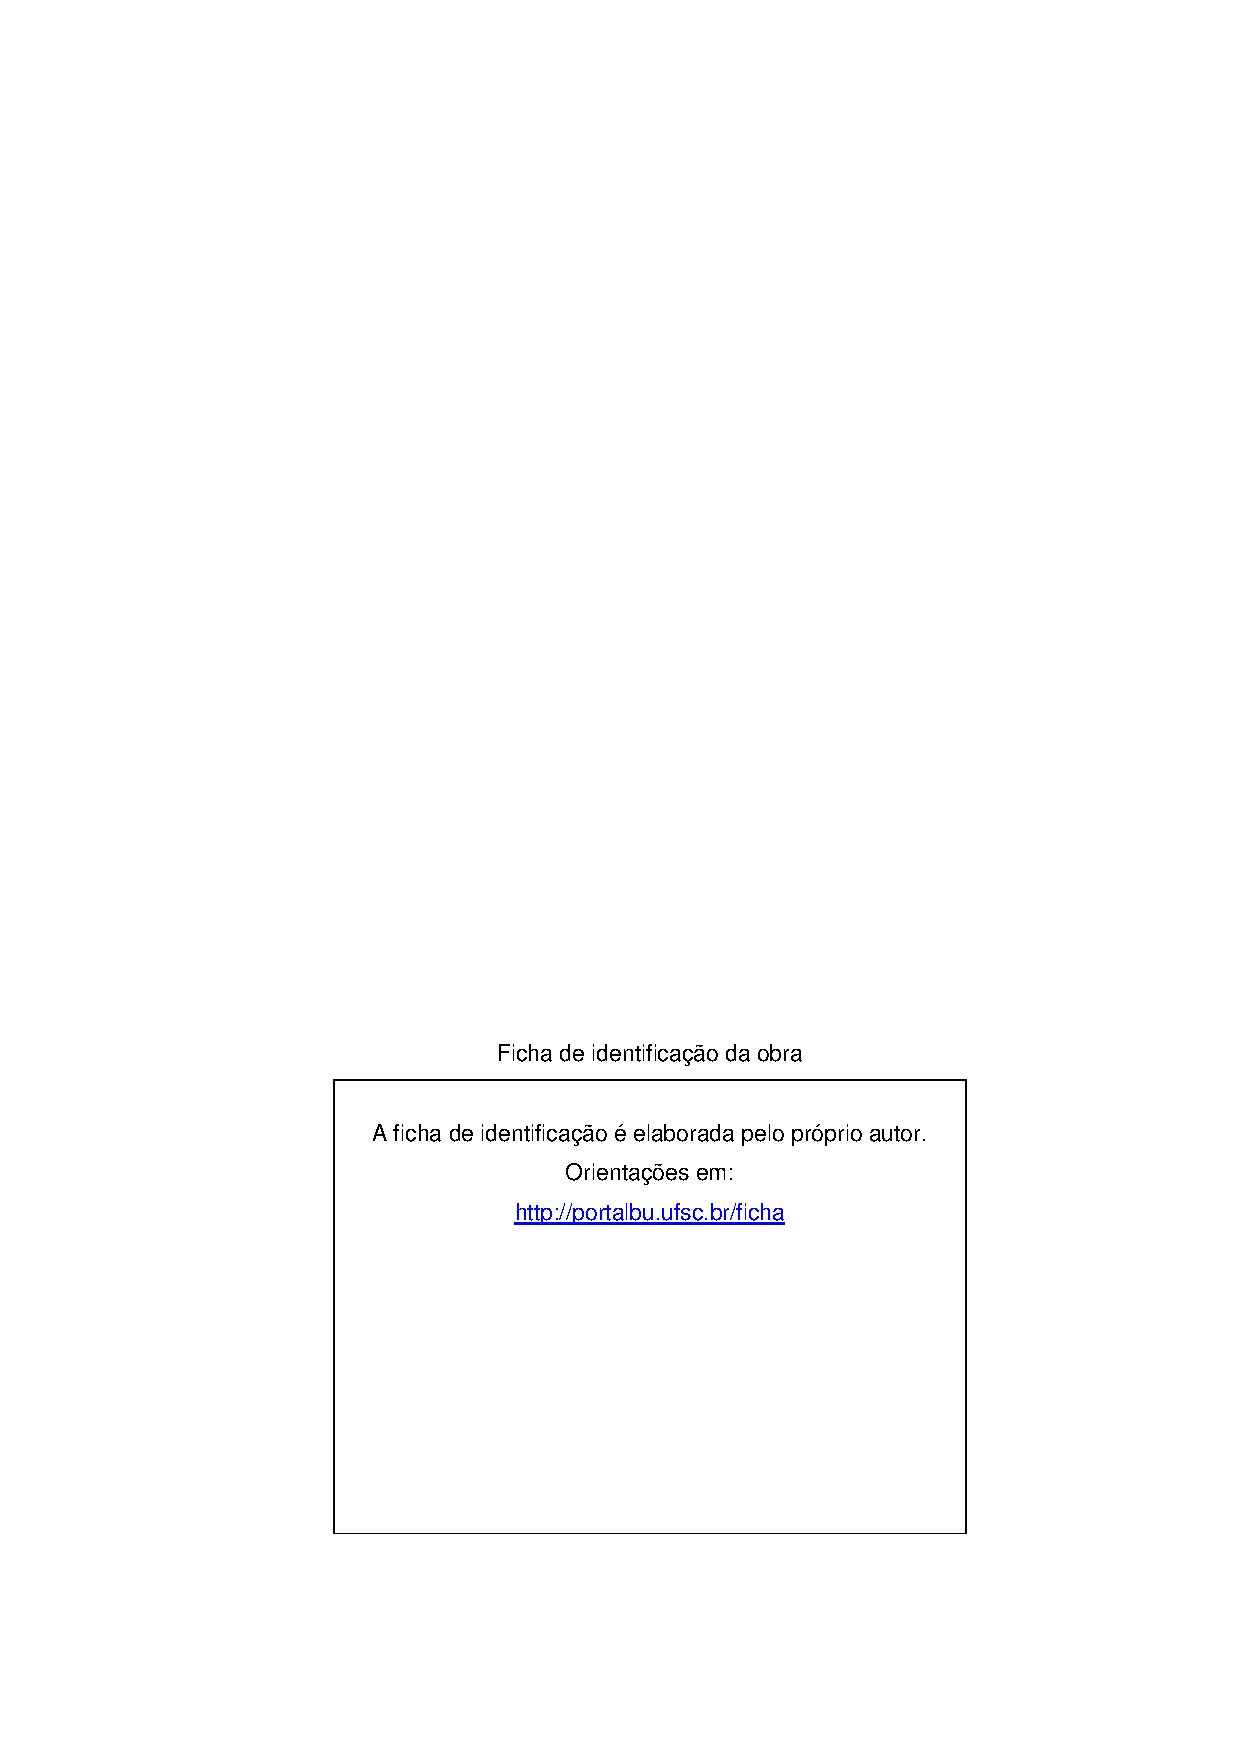
\includepdf{beforetext/Ficha_Catalografica.pdf}
\end{fichacatalografica}
% ---

% ---
% Inserir folha de aprovação
% ---
\begin{folhadeaprovacao}
	\OnehalfSpacing
	\centering
	\imprimirautor\\%
	\vspace*{10pt}		
	\textbf{\imprimirtitulo}%
	\ifnotempty{\imprimirsubtitulo}{:~\imprimirsubtitulo}\\%
	%		\vspace*{31.5pt}%3\baselineskip
	\vspace*{\baselineskip}
	%\begin{minipage}{\textwidth}
	% ~do~\imprimirprograma~do~\imprimircentro~da~\imprimirinstituicao~para~a~obtenção~do~título~de~\imprimirformacao.
	Este~\imprimirtipotrabalho~foi julgado adequado para obtenção do Título de “\imprimirformacao” e aprovado em sua forma final pelo~\imprimirprograma. \\
		\vspace*{\baselineskip}
	\imprimirlocal, \imprimirdata. \\
	\vspace*{2\baselineskip}
	\assinatura{\OnehalfSpacing\imprimircoordenador \\ \imprimircoordenadorRotulo~do Curso}
	\vspace*{2\baselineskip}
	\textbf{Banca Examinadora:} \\
	\vspace*{\baselineskip}
	\assinatura{\OnehalfSpacing\imprimirorientador \\ \imprimirorientadorRotulo}
	%\end{minipage}%
	\vspace*{\baselineskip}
	\assinatura{Prof.(a) xxxx, Dr(a).\\
	Avaliador(a) \\
	Instituição xxxx}

	\vspace*{\baselineskip}
	\assinatura{Prof.(a) xxxx, Dr(a).\\
	Avaliador(a) \\
	Instituição xxxx}


\end{folhadeaprovacao}
% ---

% ---
% Dedicatória
% ---
\begin{dedicatoria}
	\vspace*{\fill}
	\noindent
	\begin{adjustwidth*}{}{5.5cm}     
		Este trabalho é dedicado aos meus colegas de classe e aos meus queridos pais.
	\end{adjustwidth*}
\end{dedicatoria}
% ---

% ---
% Agradecimentos
% ---
\begin{agradecimentos}
	Inserir os agradecimentos aos colaboradores à execução do trabalho. 
	
	Xxxxxxxxxxxxxxxxxxxxxxxxxxxxxxxxxxxxxxxxxxxxxxxxxxxxxxxxxxxxxxxxxxxxxx. 
\end{agradecimentos}
% ---

% ---
% Epígrafe
% ---
\begin{epigrafe}
	\vspace*{\fill}
	\begin{flushright}
		\textit{``Texto da Epígrafe.\\
			Citação relativa ao tema do trabalho.\\
			É opcional. A epígrafe pode também aparecer\\
			na abertura de cada seção ou capítulo.\\
			Deve ser elaborada de acordo com a NBR 10520.''\\
			(Autor da epígrafe, ano)}
	\end{flushright}
\end{epigrafe}
% ---

% ---
% RESUMOS
% ---

% resumo em português
\setlength{\absparsep}{18pt} % ajusta o espaçamento dos parágrafos do resumo
\begin{resumo}
	\SingleSpacing
Um fluxo de trabalho (\textit{workflow}) especifica um processo envolvendo encadeamento de tarefas e fluxo de informações entre elas para alcançar um objetivo de negócio. A orquestração de um \textit{workflow} automatiza e gerencia a execução de uma instância de processo de acordo com a especificação do \textit{workflow}, usando um \textit{software} de orquestração. O orquestrador invoca recursos humanos e/ou de TI apropriados para executar cada tarefa, coordenar a execução das mesmas de acordo com o encadeamento especificado e reportar eventuais problemas encontrados durante a execução. Este trabalho de conclusão de curso está no contexto do projeto de pesquisa CÉOS, executado pela Universidade Federal de Santa Catarina (UFSC), em parceria com o Ministério Público de Santa Catarina (MPSC). O projeto CÉOS tem o objetivo de desenvolver \textit{workflows} para análise e processamento de dados em grande escala a fim de automatizar a extração de conhecimento e aumentar a eficiência das decisões tomadas em atividades do MPSC. Neste trabalho, será especificado e implementado um fluxo de trabalho para extração, transformação e carga (\textit{extract, transform, load} - ETL) de dados referentes a licitações e compras feitas pela Prefeitura Municipal de Florianópolis. O fluxo será orquestrado pelo Airflow de acordo com grafos acíclicos direcionados (\textit{directed acyclic graph} - DAG) especificados na plataforma. Os resultados serão avaliados usando métricas referentes à quantidade e qualidade dos dados, a frequência de erros e o tempo de execução dos processos de ETL.
	
	\textbf{Palavras-chave}: Extração, transformação e carga de dados. Dados abertos. Licitações.
\end{resumo}

% resumo em inglês
\begin{resumo}[Abstract]
	\SingleSpacing
	\begin{otherlanguage*}{english}
		Resumo traduzido para outros idiomas, neste caso, inglês. Segue o formato do resumo feito na língua vernácula. As palavras-chave traduzidas, versão em língua estrangeira, são colocadas abaixo do texto precedidas pela expressão “Keywords”, separadas por ponto.
		
		\textbf{Keywords}: Keyword 1. Keyword 2. Keyword 3.
	\end{otherlanguage*}
\end{resumo}

%% resumo em francês 
%\begin{resumo}[Résumé]
% \begin{otherlanguage*}{french}
%    Il s'agit d'un résumé en français.
% 
%   \textbf{Mots-clés}: latex. abntex. publication de textes.
% \end{otherlanguage*}
%\end{resumo}
%
%% resumo em espanhol
%\begin{resumo}[Resumen]
% \begin{otherlanguage*}{spanish}
%   Este es el resumen en español.
%  
%   \textbf{Palabras clave}: latex. abntex. publicación de textos.
% \end{otherlanguage*}
%\end{resumo}
%% ---

{%hidelinks
	\hypersetup{hidelinks}
	% ---
	% inserir lista de ilustrações
	% ---
	\pdfbookmark[0]{\listfigurename}{lof}
	\listoffigures*
	\cleardoublepage
	% ---
	
	% ---
	% inserir lista de quadros
	% ---
	\pdfbookmark[0]{\listofquadrosname}{loq}
	\listofquadros*
	\cleardoublepage
	% ---
	
	% ---
	% inserir lista de tabelas
	% ---
	\pdfbookmark[0]{\listtablename}{lot}
	\listoftables*
	\cleardoublepage
	% ---
	
	% ---
	% inserir lista de abreviaturas e siglas (devem ser declarados no preambulo)
	% ---
	\imprimirlistadesiglas
	% ---
	
	% ---
	% inserir lista de símbolos (devem ser declarados no preambulo)
	% ---
	\imprimirlistadesimbolos
	% ---
	
	% ---
	% inserir o sumario
	% ---
	\pdfbookmark[0]{\contentsname}{toc}
	\tableofcontents*
	\cleardoublepage
	
}%hidelinks
% ---
% ---
% Capa
% ---
\imprimircapa
% ---

% ---
% Folha de rosto
% (o * indica que haverá a ficha bibliográfica)
% ---
\imprimirfolhaderosto*
% ---

% ---
% Inserir a ficha bibliografica
% ---
% http://ficha.bu.ufsc.br/
\begin{fichacatalografica}
	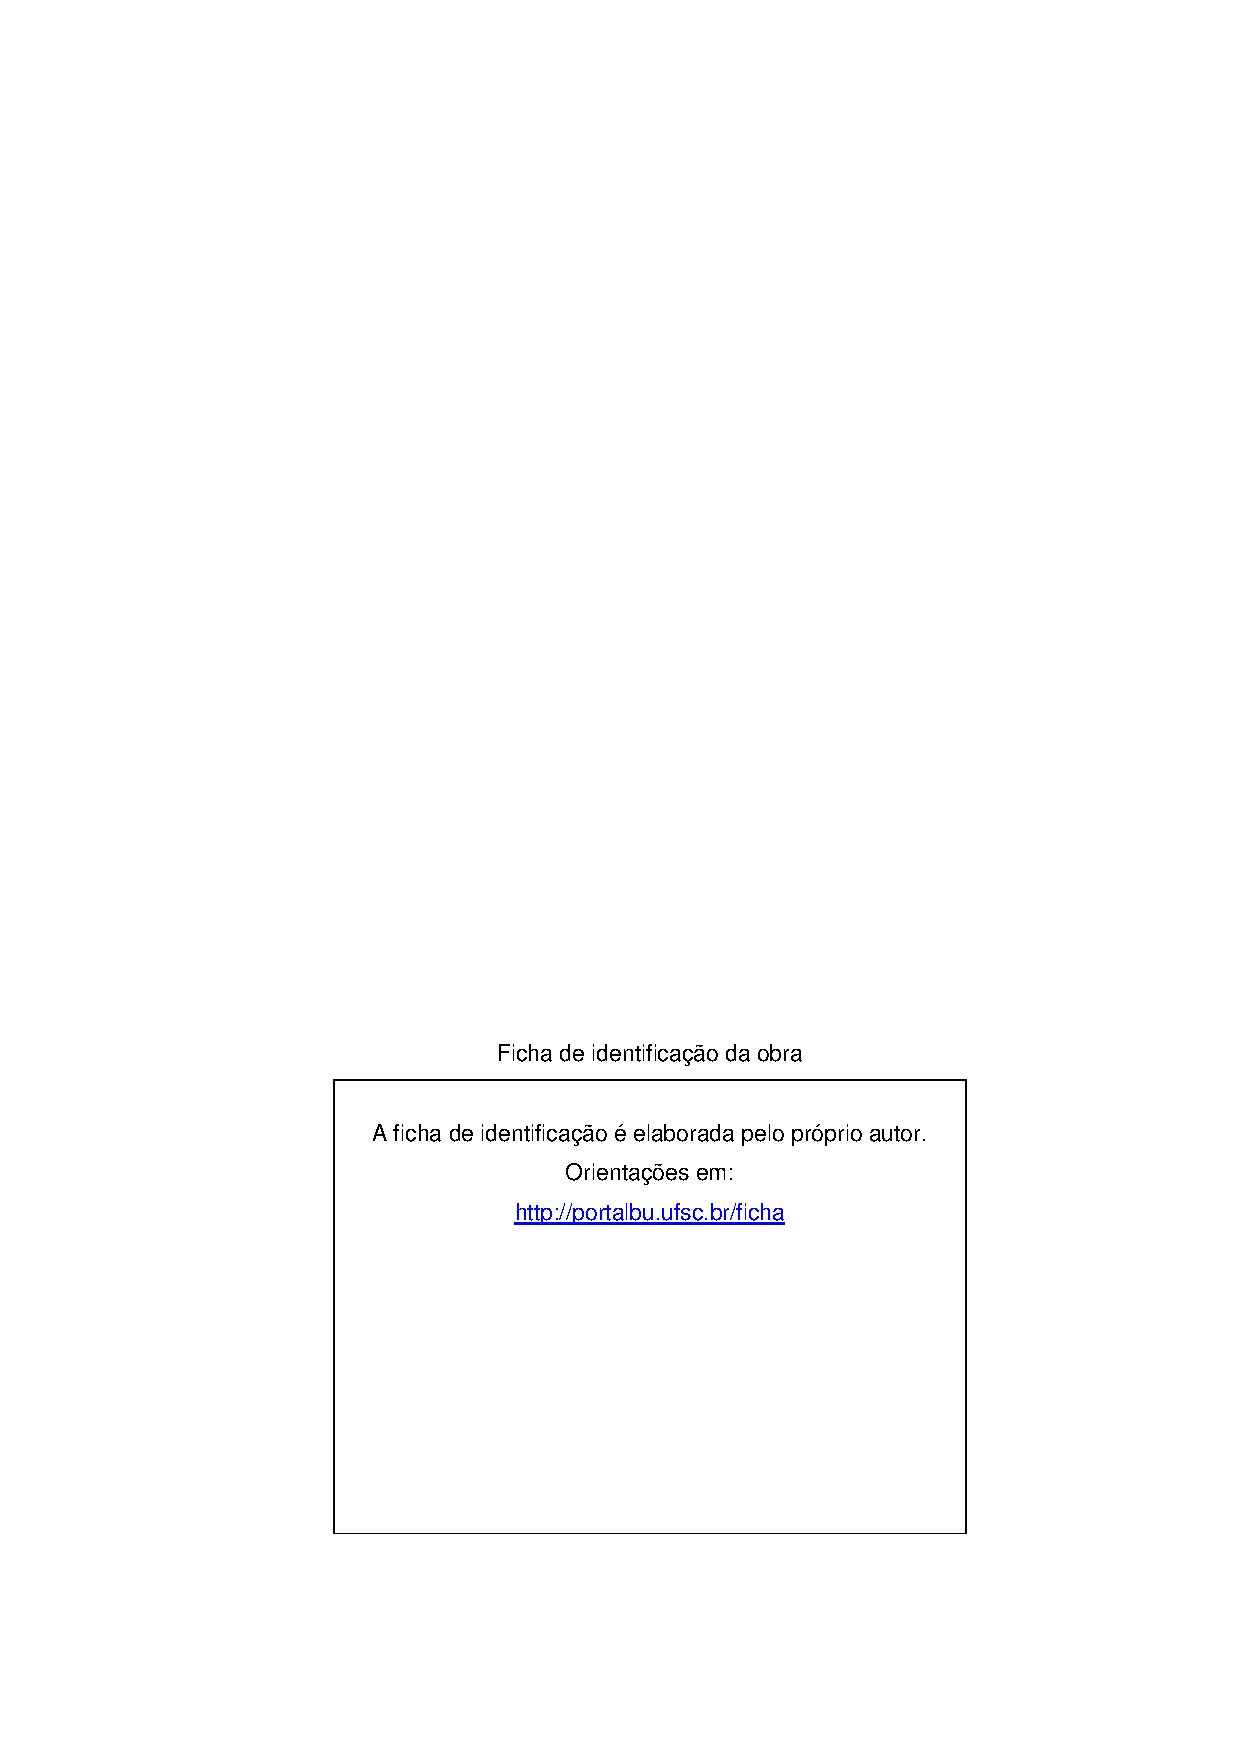
\includepdf{beforetext/Ficha_Catalografica.pdf}
\end{fichacatalografica}
% ---

% ---
% Inserir folha de aprovação
% ---
\begin{folhadeaprovacao}
	\OnehalfSpacing
	\centering
	\imprimirautor\\%
	\vspace*{10pt}		
	\textbf{\imprimirtitulo}%
	\ifnotempty{\imprimirsubtitulo}{:~\imprimirsubtitulo}\\%
	%		\vspace*{31.5pt}%3\baselineskip
	\vspace*{\baselineskip}
	%\begin{minipage}{\textwidth}
	% ~do~\imprimirprograma~do~\imprimircentro~da~\imprimirinstituicao~para~a~obtenção~do~título~de~\imprimirformacao.
	Este~\imprimirtipotrabalho~foi julgado adequado para obtenção do Título de “\imprimirformacao” e aprovado em sua forma final pelo~\imprimirprograma. \\
		\vspace*{\baselineskip}
	\imprimirlocal, \imprimirdata. \\
	\vspace*{2\baselineskip}
	\assinatura{\OnehalfSpacing\imprimircoordenador \\ \imprimircoordenadorRotulo~do Curso}
	\vspace*{2\baselineskip}
	\textbf{Banca Examinadora:} \\
	\vspace*{\baselineskip}
	\assinatura{\OnehalfSpacing\imprimirorientador \\ \imprimirorientadorRotulo}
	%\end{minipage}%
	\vspace*{\baselineskip}
	\assinatura{Profa. Carina Friedrich Dorneles, Dra.\\
	Avaliadora \\
	Universidade Federal de Santa Catarina}

	\vspace*{\baselineskip}
	\assinatura{Prof. Ronaldo dos Santos Mello, Dr.\\
	Avaliador \\
	Universidade Federal de Santa Catarina}


\end{folhadeaprovacao}
% ---

% ---
% Dedicatória
% ---
\begin{dedicatoria}
	\vspace*{\fill}
	\noindent
	\begin{adjustwidth*}{}{5.5cm}     
		Este trabalho é dedicado aos meus colegas de classe e aos meus queridos pais.
	\end{adjustwidth*}
\end{dedicatoria}
% ---

% ---
% Agradecimentos
% ---
\begin{agradecimentos}
	Inserir os agradecimentos aos colaboradores à execução do trabalho. 
	
	Xxxxxxxxxxxxxxxxxxxxxxxxxxxxxxxxxxxxxxxxxxxxxxxxxxxxxxxxxxxxxxxxxxxxxx. 
\end{agradecimentos}
% ---

% ---
% Epígrafe
% ---
\begin{epigrafe}
	\vspace*{\fill}
	\begin{flushright}
		\textit{``Texto da Epígrafe.\\
			Citação relativa ao tema do trabalho.\\
			É opcional. A epígrafe pode também aparecer\\
			na abertura de cada seção ou capítulo.\\
			Deve ser elaborada de acordo com a NBR 10520.''\\
			(Autor da epígrafe, ano)}
	\end{flushright}
\end{epigrafe}
% ---

% ---
% RESUMOS
% ---

% resumo em português
\setlength{\absparsep}{18pt} % ajusta o espaçamento dos parágrafos do resumo
\begin{resumo}
	\SingleSpacing
Um fluxo de trabalho (\textit{workflow}) especifica um processo envolvendo encadeamento de tarefas e fluxo de informações entre elas para alcançar um objetivo de negócio. A orquestração de um \textit{workflow} automatiza e gerencia a execução de uma instância de processo de acordo com a especificação do \textit{workflow}, usando um \textit{software} de orquestração. O orquestrador invoca recursos humanos e/ou de TI apropriados para executar cada tarefa, coordenar a execução das mesmas de acordo com o encadeamento especificado e reportar eventuais problemas encontrados durante a execução. Este trabalho de conclusão de curso está no contexto do projeto de pesquisa CÉOS, executado pela Universidade Federal de Santa Catarina (UFSC), em parceria com o Ministério Público de Santa Catarina (\glsxtrshort{MPSC}). O projeto CÉOS tem o objetivo de desenvolver \textit{workflows} para análise e processamento de dados em grande escala a fim de automatizar a extração de conhecimento e aumentar a eficiência das decisões tomadas em atividades do \glsxtrshort{MPSC}. Neste trabalho, é especificado e implementado um fluxo de trabalho para extração, transformação e carga (\textit{extract, transform, load} - \glsxtrshort{ETL}) de dados referentes a licitações e compras feitas pela \glsxtrlong{PMF}. O fluxo é orquestrado pelo Airflow de acordo com grafos acíclicos direcionados (\textit{directed acyclic graph} - \glsxtrshort{DAG}) especificados na plataforma. Os resultados são avaliados usando métricas referentes à quantidade e qualidade dos dados, a frequência de erros e o tempo de execução dos processos de \glsxtrshort{ETL}.
	
	\textbf{Palavras-chave}: Extração, transformação e carga de dados. Dados abertos. Licitações.
\end{resumo}

% resumo em inglês
\begin{resumo}[Abstract]
	\SingleSpacing
	\begin{otherlanguage*}{english}
		A workflow specifies a process involving the chaining of tasks and the flow of information between them in order to achieve a business objective. The orchestration of a workflow automates and manages the execution of a process instance according to the workflow specification, using orchestration software. The orchestrator invokes appropriate human and/or IT resources to execute each task, coordinates their execution according to the specified chaining, and reports any issues encountered during execution. This undergraduate thesis is part of the CÉOS research project, carried out by the Federal University of Santa Catarina (UFSC) in partnership with the Public Prosecutor's Office of Santa Catarina (\glsxtrshort{MPSC}). The CÉOS project aims to develop workflows for the analysis and processing of large-scale data in order to automate knowledge extraction and improve the efficiency of decision-making processes within \glsxtrshort{MPSC} activities. In this work, a workflow is specified and implemented for extract, transform, and load (\glsxtrshort{ETL}) processes involving data related to bidding and procurement carried out by the Municipality of Florianópolis. The workflow is orchestrated by Airflow according to directed acyclic graphs (\glsxtrshort{DAG}s) specified in the platform. The results are evaluated using metrics related to data quantity and quality, error frequency, and \glsxtrshort{ETL} process execution time.
		
		\textbf{Keywords}: Extraction, transformation and loading of data. Open data. Public procurement.
	\end{otherlanguage*}
\end{resumo}

%% resumo em francês 
%\begin{resumo}[Résumé]
% \begin{otherlanguage*}{french}
%    Il s'agit d'un résumé en français.
% 
%   \textbf{Mots-clés}: latex. abntex. publication de textes.
% \end{otherlanguage*}
%\end{resumo}
%
%% resumo em espanhol
%\begin{resumo}[Resumen]
% \begin{otherlanguage*}{spanish}
%   Este es el resumen en español.
%  
%   \textbf{Palabras clave}: latex. abntex. publicación de textos.
% \end{otherlanguage*}
%\end{resumo}
%% ---

{%hidelinks
	\hypersetup{hidelinks}
	% ---
	% inserir lista de ilustrações
	% ---
	\pdfbookmark[0]{\listfigurename}{lof}
	\listoffigures*
	\cleardoublepage
	% ---
	
	% ---
	% inserir lista de quadros
	% ---
	%\pdfbookmark[0]{\listofquadrosname}{loq}
	%\listofquadros*
	%\cleardoublepage
	% ---
	
	% ---
	% inserir lista de tabelas
	% ---
	\pdfbookmark[0]{\listtablename}{lot}
	\listoftables*
	\cleardoublepage
	% ---
	
	% ---
	% inserir lista de abreviaturas e siglas (devem ser declarados no preambulo)
	% ---
	\imprimirlistadesiglas
	% ---
	
	% ---
	% inserir lista de símbolos (devem ser declarados no preambulo)
	% ---
	%\imprimirlistadesimbolos
	% ---
	
	% ---
	% inserir o sumario
	% ---
	\pdfbookmark[0]{\contentsname}{toc}
	\tableofcontents*
	\cleardoublepage
	
}%hidelinks
% ---
% ---

% ----------------------------------------------------------
% ELEMENTOS TEXTUAIS
% ----------------------------------------------------------
\textual

% ---
% 1 - Introdução
% ---
% ----------------------------------------------------------
\chapter{Introdução}
% ----------------------------------------------------------

O uso de plataformas de orquestração de \textit{workflows} é imprescindível para gerenciar aplicações com uso intenso de dados, como \textit{data warehouses}. \cite{hollingsworth1995workflow} define \textit{workflow} como a automação informatizada total ou parcial de um processo de negócio e afirma que um sistema de gerenciamento de \textit{workflows} deve fornecer suporte a três tipos de funções: (i) as funções \textit{build-time}, referentes à definição e modelagem do processo de \textit{workflow}; (ii) as funções \textit{run-time control}, que envolvem o sequenciamento da execução das atividades e (iii) as interações de \textit{run-time} entre os usuários e as aplicações de TI que processam os passos das atividades.

\textit{Workflows} são frequentemente utilizados para implementar processos de extração, transformação e carga (em inglês \textit{extraction-transformation-loading} - \glsxtrshort{ETL}) de dados. \cite{vassiliadis2002conceptual} fornecem uma descrição generalizada de processos \glsxtrshort{ETL}. Dados são obtidos de fontes como bancos de dados relacionais ou arquivos por rotinas de extração. Depois, os dados são propagados a uma ou mais \textit{data staging areas}, onde são transformados a um formato homogêneo. Por fim, os dados formatados são inseridos em um banco de dados, muitas vezes no modelo multidimensional de um \textit{data warehouse}.

O Apache Airflow é uma plataforma de orquestração de \textit{workflows} de código aberto utilizada para implementar e manter \textit{pipelines} de dados. No Airflow, \textit{workflows} são definidos por grafos acíclicos direcionados, ou \glsxtrshort{DAG}s (do inglês \textit{directed acyclic graph}). \glsxtrshort{DAG}s são \textit{scripts} escritos na linguagem Python, utilizando construções básicas como operadores. \glsxtrshort{DAG}s definem as tarefas a serem executadas, as quais podem ser especificadas por operadores, e relações que indicam a ordem de execução e as dependências entre tarefas. Estes componentes formarão a \textit{pipeline} do Airflow \cite{finnigan2021building}.

Este trabalho busca descrever, de forma detalhada, o desenvolvimento de um fluxo de \glsxtrshort{ETL} desde a obtenção de dados até o processamento e carga dos dados. Primeiramente, duas fontes são acessadas: (i) um \textit{web scraper} que acessa o Portal da Transparência da Controladoria-Geral da União e extrai dados referentes a contratos de compras feitas por órgãos do município de Florianópolis e (ii) um \textit{script} que faz uma requisição da \glsxtrshort{API} de dados públicos do Portal de Transparência da \glsxtrlong{PMF} buscando registros de contratos e licitações, incluindo número, nome e CPF/CNPJ do fornecedor, período de vigência e valor monetário. Depois, a orquestração dos fluxos de trabalho é implementada por meio da execução de processos de acordo com especificações desses fluxos na forma de \glsxtrshort{DAG}s no Airflow. Esses processos visam limpar e padronizar os dados em
um formato adequado para o armazenamento. A análise exploratória e a visualização dos dados são feitas com a geração de tabelas, gráficos e eventualmente grafos, que permitem analisar a estrutura e a distribuição dos dados, tais como os custos dos contratos para identificar irregularidades. O desempenho do fluxo de \glsxtrshort{ETL} é avaliado com base nos tempos de execução das tarefas dos \glsxtrshort{DAG}s, na quantidade de dados tratados e na quantidade de erros encontrados durante e após a transformação.

% ----------------------------------------------------------
\section{Objetivos}
% ----------------------------------------------------------
% ----------------------------------------------------------
\subsection{Objetivo Geral}
% ----------------------------------------------------------

O objetivo geral deste trabalho é orquestrar um fluxo de extração, transformação e carregamento de dados relacionados a compras feitas por órgãos públicos do município de Florianópolis, com o intuito de suprir dados para  analisar os gastos com as compras no projeto CÉOS. Os resultados serão avaliados através de uma análise exploratória de dados resultantes em tabelas e gráficos, que permitirão visualizar suas distribuições. Também serão medidos os tempos de execução das tarefas e as quantidades de erros encontrados nos dados, tratados ou não dentro nos processos de \glsxtrshort{ETL} implementados e avaliados.

% ----------------------------------------------------------
\subsection{Objetivos Específicos}
% ----------------------------------------------------------

Os objetivos específicos são:
\begin{enumerate}
    \item Estudar conceitos de orquestração de fluxos de \glsxtrshort{ETL}.
    \item Desenvolver códigos para obtenção de dados utilizando métodos de web scraping e requisições em uma \glsxtrshort{API} pública.
    \item Construir \glsxtrshort{DAG}s para implementar o fluxo de \glsxtrshort{ETL}, que padronizará os dados em um formato adequado.
    \item Orquestrar processos de \glsxtrshort{ETL} usando as \glsxtrshort{DAG}s construídas, coletando métricas para avaliar sua capacidade, desempenho e custos computacionais.
    \item Utilizar ferramentas de análise e visualização de dados para gerar tabelas e gráficos sobre as distribuições dos dados carregados e a análise dos custos computacionais dos processos de \glsxtrshort{ETL}.
\end{enumerate}

% ----------------------------------------------------------
\section{Metodologia}
% ----------------------------------------------------------

A metodologia adotada neste trabalho é estruturada em três etapas principais, contemplando desde o estudo preliminar até a implementação e análise dos dados extraídos.

A primeira etapa consiste em um levantamento teórico sobre os conceitos, ferramentas e práticas envolvidas na orquestração de \textit{pipelines} de \glsxtrshort{ETL} (\textit{extraction-transformation-loading}) utilizando o Apache Airflow. Foram reunidos artigos científicos, publicações técnicas e documentação especializada sobre a estrutura e implementação de \glsxtrshort{DAG}s no Airflow, bem como sobre métodos de \textit{web scraping}, a fim de possibilitar a extração de dados não estruturados diretamente de páginas da Web.

Na segunda etapa, foi realizada a implementação dos \textit{scripts} responsáveis pela extração de dados por meio de \textit{web scraping} e requisições a \glsxtrshort{API}s \glsxtrshort{REST}. Os dados obtidos a partir dos \textit{endpoints} públicos disponibilizados no Portal de Transparência da \glsxtrlong{PMF} estavam incompletos, o que tornou necessário consultar os \textit{endpoints} internos do sistema para extrair os dados faltantes. Após este processo, realizou-se uma análise exploratória dos dados, consistindo na geração de gráficos para visualização de possíveis \textit{outliers} entre os registros e na construção de um dicionário de dados e, subsequentemente, a modelagem de um esquema para bancos de dados relacionais.

A terceira e última etapa envolve a orquestração completa do fluxo \glsxtrshort{ETL} no ambiente do Airflow, seguida da análise dos dados carregados. Foram realizados testes de execução e ajustes nos fluxos com base na avaliação de métricas, como tempo de execução e ocorrência de erros, e a partir dos dados transformados, foram geradas tabelas e gráficos mais detalhados, permitindo a análise mais complexa.

% ----------------------------------------------------------
\section{Organização do documento}
% ----------------------------------------------------------

O trabalho está organizado da seguinte maneira: o Capítulo 2 apresenta os fundamentos de conceitos e tecnologias utilizados para desenvolver o trabalho. No Capítulo 3, faz-se uma comparação de trabalhos que abordam temas semelhantes a este. O Capítulo 4 descreve os processos de análise exploratória dos dados e implementação do fluxo \glsxtrshort{ETL}. No Capítulo 5, são discutidos os resultados obtidos a partir da análise. Finalmente, o Capítulo 6 apresenta conclusões e temas para trabalhos futuros.
% ---

% ---
% 2 - Capítulo 2
% ---
% ----------------------------------------------------------
\chapter{Fundamentos}\label{cap:fundamentos}
% ----------------------------------------------------------
Neste capítulo são apresentados conceitos teóricos relacionados ao trabalho. Na Seção \ref{sec:etl_dados}, apresenta-se o processo de extração, transformação e carga de dados com as definições de cada etapa do processo. A Seção \ref{sec:airflow} apresenta a plataforma de software Apache Airflow, utilizada para orquestrar fluxos de trabalho, além de seus componentes e sua interface gráfica. A Seção \ref{sec:transparencia} apresenta o conceito de dados abertos e iniciativas de transparência governamental em nível federal e municipal; na Subseção \ref{ssec:licitacoes_contratos}, são definidos licitações e contratos administrativos de acordo com a Lei 14.133/2021. Por fim, a Seção \ref{sec:dados_abertos} apresenta a \glsxtrshort{API} de compras públicas da \glsxtrlong{PMF} e define um dicionário de dados a partir dos resultados de consultas feitas.

% ----------------------------------------------------------
\section{Extração, transformação e carga (\glsxtrshort{ETL}) de dados}\label{sec:etl_dados}
% ----------------------------------------------------------

Processos de extração, transformação e carga de dados são responsáveis pela coleta, extração, limpeza, transformação integração e carga de dados de uma ou mais fontes para um sistema destino, tal como um \textit{data warehouse}. De acordo com \cite{vassiliadis2009extraction}, qualquer programa que filtra registros, calcula novos valores e alimenta uma fonte de dados diferente da original pode ser considerado um programa de \glsxtrshort{ETL}.

\cite{vassiliadis2009extraction} descrevem o fluxo de trabalho de um processo \glsxtrshort{ETL} como um grafo acíclico direcionado, no qual as tarefas executadas são análogas aos nodos do grafo e as relações entre entradas e saídas são análogas às arestas do grafo.

% \begin{figure}[htb]
% 	\caption{\label{fig:Fig_1}Exemplo de fluxo de trabalho ETL.}
% 	\begin{center}
% 		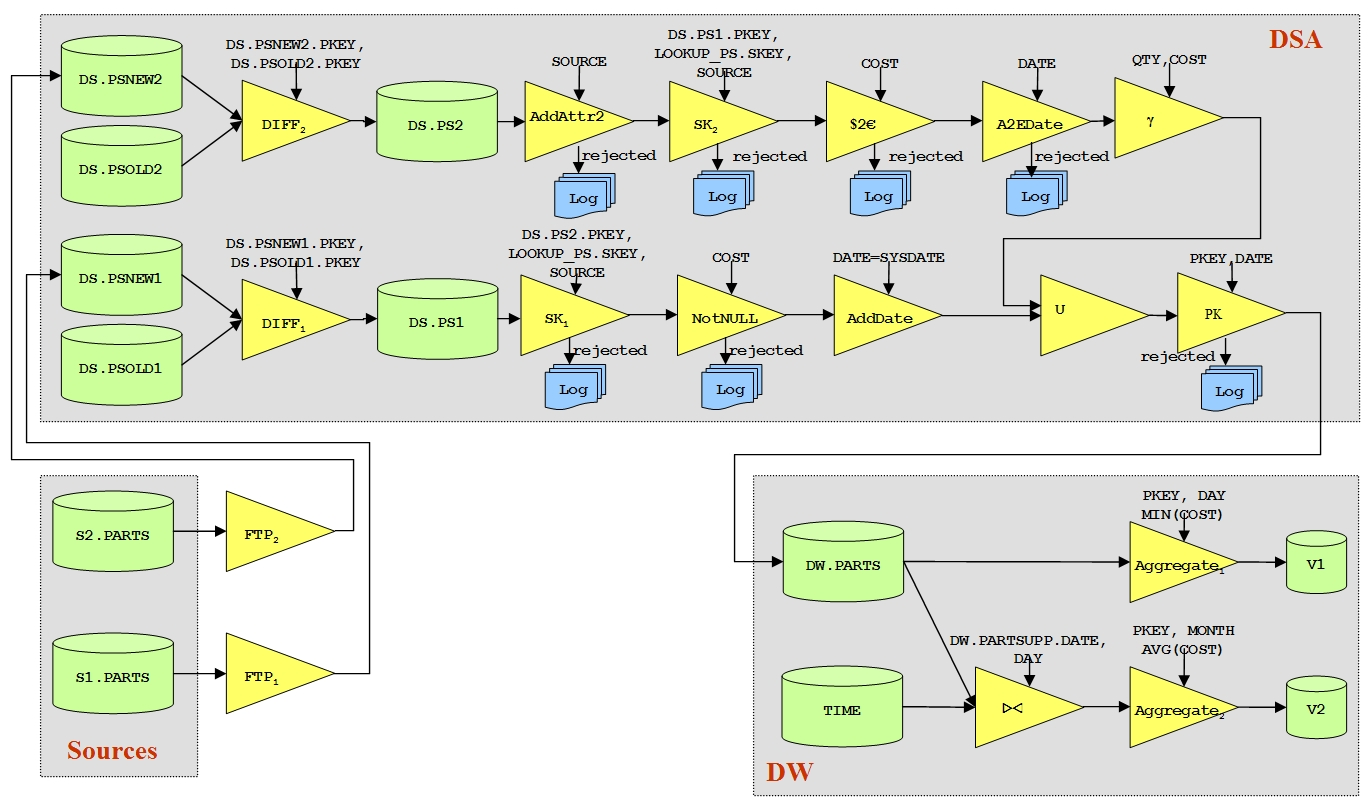
\includegraphics[scale=0.32]{images/etl.png}
% 	\end{center}
% 	\fonte{\cite{vassiliadis2009extraction}}
% \end{figure}

A primeira etapa do processo \glsxtrshort{ETL} é a extração. Nesta, dados são obtidos de fontes, que podem estar no formato de documentos de texto, planilhas, páginas da Web ou \textit{streaming}. Geralmente, busca-se extrair apenas os dados que foram inseridos ou atualizados após a última execução do processo.

A segunda etapa é a transformação. Esta etapa envolve a normalização, formatação, padronização e enriquecimento de dados visando resolver problemas em nível de esquema (conflitos de nomeação de objetos ou diferenças na estruturação de dados entre fontes e o \textit{data warehouse}) e em nível de registro (registros duplicados, contraditórios, ou com referências temporais diferentes).

A terceira e última etapa é a carga. Os dados transformados são carregados nas tabelas apropriadas do \textit{data warehouse}, onde servirão como base para processos de análise, visualização e apoio a tomadas de decisões.

% ----------------------------------------------------------
\section{Apache Airflow}\label{sec:airflow}
% ----------------------------------------------------------

O Apache Airflow é uma plataforma de código aberto utilizada para orquestrar e monitorar fluxos de trabalho no formato de grafos acíclicos direcionados, ou \glsxtrshort{DAG}s. No Airflow, os \glsxtrshort{DAG}s são definidos por meio de arquivos, ou \textit{scripts} na linguagem Python que descrevem as tarefas a serem executadas e as dependências entre as tarefas, além de metadados com configurações específicas. O Airflow interpreta estes \textit{scripts} e modela a estrutura das \glsxtrshort{DAG}s, executando as tarefas de acordo com o intervalo de tempo agendado nos metadados.

De acordo com \cite{de2021data}, o uso de código em Python para definir \glsxtrshort{DAG}s garante flexibilidade ao desenvolvedor, pois qualquer função implementada em Python pode ser executada pelo Airflow. Assim, é possível importar funções de bibliotecas externas e criar fluxos de trabalho altamente escaláveis que estabelecem comunicações entre diversos serviços.

\cite{de2021data} afirmam que o Airflow pode ser dividido em três componentes: (i) o escalonador, que lê os \textit{scripts} de \glsxtrshort{DAG}s desenvolvidos e obtém as tarefas, dependências e intervalos de execução, verifica se o intervalo de cada \glsxtrshort{DAG} passou e, se este for o caso, adiciona as respectivas tarefas à fila de execução, (ii) os trabalhadores, que obtêm tarefas escalonadas da fila e as executam em paralelo e (iii) o servidor \textit{web}, que fornece uma interface com representações visuais das \glsxtrshort{DAG}s e permite que o usuário monitore os resultados das tarefas executadas.

\begin{figure}[hb!]
	\caption{\label{fig:Fig_2}Diagrama mostrando os componentes do Airflow.}
	\begin{center}
		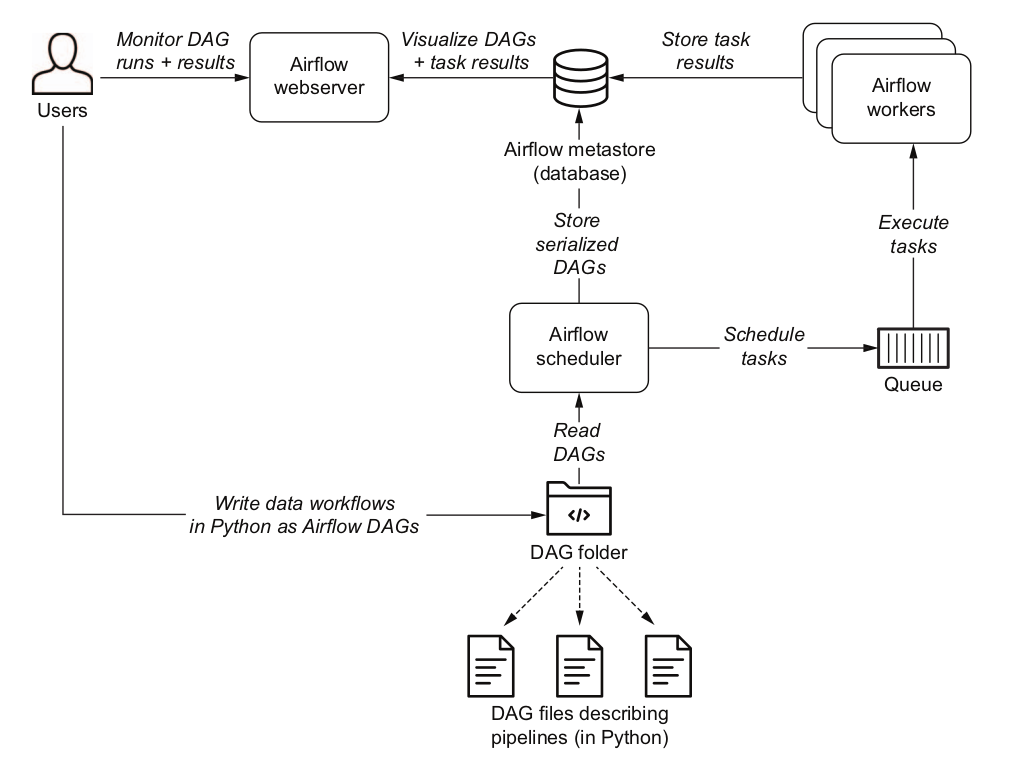
\includegraphics[scale=0.55]{images/airflow-components.png}
	\end{center}
	\fonte{\cite{de2021data}}
\end{figure}

A interface \textit{web} do Airflow oferece diferentes modos de visualização das \glsxtrshort{DAG}s. O modo \textit{graph view} (visualização de grafo) mostra um esquema contendo as tarefas e as respectivas dependências, enquanto o modo \textit{tree view} (visualização de árvore) mostra o histórico dos resultados das execuções das \glsxtrshort{DAG}s, também permitindo verificar detalhes de tarefas específicas, com indicadores de status e \textit{logs} de textos com informações referentes a possíveis erros de execução.

\begin{figure}[h!]
	\caption{\label{fig:teste}Exemplo básico de \textit{graph view} de uma \glsxtrshort{DAG} no Airflow.}
	\begin{center}
		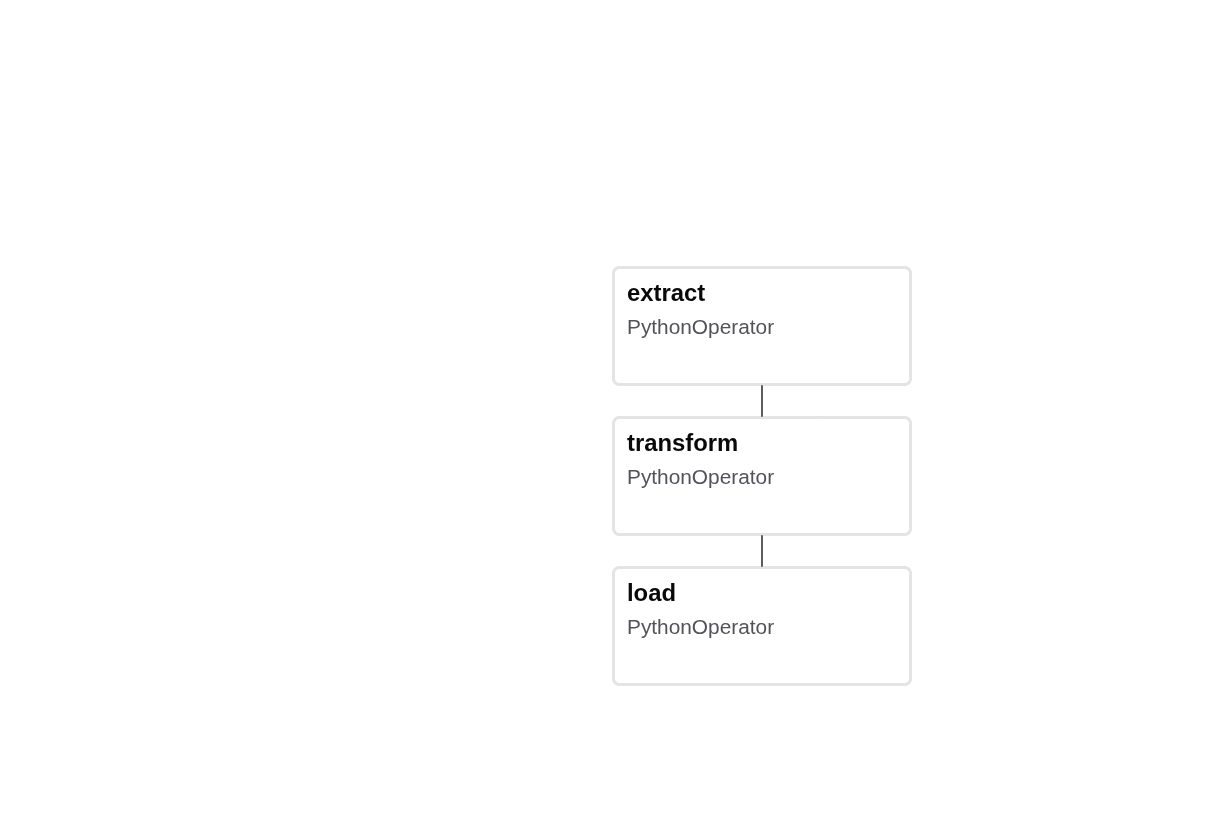
\includegraphics[trim={11cm 6cm 0 9cm},width=\textwidth]{images/tutorial_dag-graph (2).png}
	\end{center}
	\fonte{Elaborada pelo autor.}
\end{figure}

% ----------------------------------------------------------
\section{Transparência e dados abertos}\label{sec:transparencia}
% ----------------------------------------------------------

\cite{possamai2020transparencia} afirmam que dados abertos governamentais são dados públicos produzidos ou curados por órgãos estatais, padronizados em formatos abertos e legíveis por máquina, como \glsxtrshort{JSON} ou \glsxtrshort{XML}, e que podem ser livremente acessados e utilizados para quaisquer finalidades. A disponibilidade de dados abertos governamentais é importante para garantir a transparência com gastos públicos, incentivar a colaboração entre o cidadão e a Administração Pública e combater a corrupção.

Segundo \cite{possamai2020transparencia}, a Lei 12.527/2011 regula o acesso às informações contidas em documentos de órgãos públicos e estabelece duas formas de transparência a serem implementadas: (i) a transparência passiva, que envolve o atendimento a solicitações de informação por meio físico ou eletrônico, e (ii) a transferência ativa, referente à divulgação de um rol mínimo de informações por parte dos órgãos independentemente de requerimento. A Lei 12.527/2011 faz referência explícita aos princípios dos dados abertos em seu texto.

De acordo com \cite{nazario2012avaliaccao}, um dos principais projetos de visualização de dados abertos governamentais é o Portal de Transparência do Governo Federal, inicialmente lançado em novembro de 2004. Em concordância com a Lei Complementar 131/09, o Portal disponibiliza informações referentes a receitas, transferências e convênios recebidos, assim como despesas envolvendo processos licitatórios, contratos e gastos com diárias.

Em relação à cidade de Florianópolis, \cite{santos2021ferramenta} afirmam que a Prefeitura Municipal regulamentou o acesso à informação pública por meio do decreto 9988/12, posteriormente instituindo o Portal de Transparência de Florianópolis por meio da Lei Municipal 9.447/14. Analogamente ao Portal de Transparência do Governo Federal, o usuário possui acesso a receitas e despesas da Prefeitura e de seus órgãos.

% ----------------------------------------------------------
\subsection{Licitações e contratos administrativos}\label{ssec:licitacoes_contratos}
% ----------------------------------------------------------

\cite{tcu2023} define licitação como “o processo por meio do qual a Administração Pública convoca, sob condições estabelecidas em ato próprio (edital de licitação), interessados para apresentação de propostas relativas ao fornecimento de bens, prestação de serviços ou execução de obras”. O processo licitatório é regulamentado pela Lei 14.133/2021, cujo artigo 17 o divide em sete fases: (i) fase preparatória, (ii) divulgação do edital, (iii) apresentação de propostas e lances, (iv) julgamento, (v) habilitação, (vi) recursal e (vii) homologação.

O artigo 11 da Lei 14.133/2021 aponta como objetivos (i) garantir que seja selecionada a proposta apta a gerar o resultado de contratação mais vantajoso à Administração Pública, (ii) assegurar o tratamento isonômico e a justa competição entre os licitantes, (iii) evitar sobrepreço nas contratações e superfaturamento na execução dos contratos e (iv) incentivar a inovação e a sustentabilidade no desenvolvimento nacional.

Segundo a Lei 14.133/2021, existem cinco modalidades de licitação:
\begin{enumerate}
    \item Pregão: aquisição de bens e serviços comuns definidos pelo edital, seguindo critérios de julgamento de menor preço ou maior desconto.
    \item Concorrência: aquisição de bens e serviços especiais e de obras e serviços comuns e especiais de engenharia, utilizando critérios de julgamento de menor preço, maior desconto, melhor técnica ou conteúdo artístico, técnica e preço ou maior retorno econômico.
    \item Concurso: escolha de trabalho técnico, científico ou artístico, utilizando o critério de julgamento de melhor técnica ou conteúdo artístico e concedendo prêmio ou remuneração ao vencedor.
    \item Leilão: alienação de bens imóveis ou de bens móveis inservíveis ou legalmente apreendidos, seguindo o critério de julgamento de maior lance.
    \item Diálogo competitivo: contratação de obras, serviços e compras por meio de diálogos entre a Administração Pública e licitantes previamente selecionados, visando uma solução que atenda a uma necessidade definida.
\end{enumerate}

De acordo com \cite{tcu2023}, contratos administrativos são “aqueles firmados entre órgãos ou entidades da Administração Pública e particulares, por meio do qual se estabelece acordo de vontades, para a formação de vínculo e a estipulação de obrigações recíprocas”, que têm como objetivo principal atender a um interesse coletivo.

% ----------------------------------------------------------
\section{Dados abertos de compras públicas da \glsxtrshort{PMF}}\label{sec:dados_abertos}
% ----------------------------------------------------------

% \attention{Parágrafo inicial com descrição geral}
\urldef{\licitacoes}\url{https://transparencia.e-publica.net/epublica-portal/#/florianopolis/portal/dadosAbertos/licitacaoView}

\urldef{\contratos}\url{https://transparencia.e-publica.net/epublica-portal/#/florianopolis/portal/dadosAbertos/contratoView}

Esta seção é dividida em duas subseções. A Subseção 2.4.1 descreve a \glsxtrshort{API} de compras públicas disponível no \textit{website} do Portal de Transparência da \glsxtrlong{PMF}, o método de consulta de dados e os parâmetros de pesquisa. A Subseção 2.4.2 apresenta um dicionário de dados, no qual os conteúdos das respostas da \glsxtrshort{API} são esquematizados em tabelas.

\subsection{\glsxtrshort{API} de compras públicas da \glsxtrshort{PMF}}\label{ssec:api_compras_pmf}

O Portal de Transparência da \glsxtrlong{PMF} disponibiliza informações relacionadas a compras públicas efetuadas pela Prefeitura e as unidades gestoras que a compõem, em concordância com o princípio de dados abertos. O \textit{website} do Portal, além de mostrar listas com registros de compras, oferece uma \glsxtrshort{API} \glsxtrshort{REST} que permite ao usuário fazer requisições destes registros utilizando o formato \glsxtrshort{JSON}.

A \glsxtrshort{API} possui diversos \textit{endpoints}, dos quais são utilizados os de consulta de licitações\footnote{Disponível em: \licitacoes} e de contratos administrativos\footnote{Disponível em: \contratos}. O acesso a estes \textit{endpoints} é livre, sem necessidade de chave para autenticação.

O único método fornecido para ambos os \textit{endpoints} é o GET, que retorna dados de licitações ou contratos em formato \glsxtrshort{JSON}. Em ambos os \textit{endpoints}, é possível filtrar os resultados pelas datas inicial e final do período de busca, o código da unidade gestora responsável e o limite máximo de registros a serem retornados. Apenas as datas inicial e final são parâmetros obrigatórios.
% Os seguintes \textit{links} contêm descrições e exemplos da API:

% \url{https://transparencia.e-publica.net/epublica-portal/#/florianopolis/portal/dadosAbertos/licitacaoView?params=%7B%22mode%22:%22INFO%22%7D&entidade=2002}

% \url{https://transparencia.e-publica.net/epublica-portal/#/florianopolis/portal/dadosAbertos/contratoView?params=%7B%22mode%22:%22INFO%22%7D&entidade=2002}

\subsection{Descrição dos dados retornados}\label{ssec:descricao_dados}

A estrutura dos registros  retornados difere de acordo com os \textit{endpoints}. A \autoref{fig:json-licitacoes} apresenta a estrutura dos registros retornados pelo \textit{endpoint} Licitação. Estes registros contêm dados como o valor da licitação, datas de emissão e abertura, modalidade do processo licitatório, advogado responsável, lista de itens negociados e vencedores do processo, lista de \textit{links} a documentos relacionados, lista de empenhos e lista de contratos.

A \autoref{fig:json-contratos} mostra a estrutura dos registros retornados pelo \textit{endpoint} Contrato. Nestes registros, encontra-se dados como as datas de assinatura e início de vigência, valor total do contrato, nome do fornecedor, lista de itens e lista de empenhos.

% ... contém as seguintes propriedades ...:

\begin{figure}[htb]
    \centering
    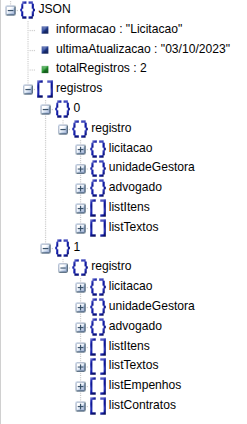
\includegraphics[width=0.36\linewidth]{images/json_licitacao_v2.png}
    \caption{Visão em árvore do \glsxtrshort{JSON} de licitações.}
    \label{fig:json-licitacoes}
\end{figure}

% <citar outros endpoints; justificar porque apenas dois>

O dicionário de dados a seguir foi desenvolvido a partir do conteúdo retornado pelo método GET da \glsxtrshort{API}. Além do cabeçalho do arquivo \glsxtrshort{JSON}, que contém metadados, são retornados elementos de dados \glsxtrshort{JSON} para as entidades \texttt{Licitação} e \texttt{Contrato administrativo}, bem como as entidades auxiliares, que representam objetos aninhados nos registros.

O \textit{Website} do Portal de Transparência da \glsxtrlong{PMF} também disponibiliza \textit{endpoints} para a consulta de receitas, despesas orçamentárias, execuções de despesa e dados da gestão de pessoal; estes não foram utilizados no trabalho, devido aos dados possuírem pouca relação ao contexto dos processos licitatórios.

Os arquivos \glsxtrshort{JSON} seguem padrões semelhantes; ambos os \textit{endpoints} consultados no trabalho retornam arquivos com as seguintes propriedades:

\newpage
\subsubsection*{Cabeçalho do \glsxtrshort{JSON}}

\begin{longtable}{|p{4cm}|p{3cm}|p{2cm}|p{6cm}|}
\hline
\textbf{Nome do Campo} & \textbf{Tipo de Dado} & \textbf{Tamanho} & \textbf{Descrição} \\
\hline
informacao & Texto & 50 & Tipo de informação retornada pela \glsxtrshort{API} (\texttt{`Licitacao'}, \texttt{`Contrato'}, \texttt{`Receita'},  \texttt{`Despesa Orçamentária'}, \texttt{`Execução de Despesa'}). \\
\hline
ultimaAtualizacao & Data & - & Data da última atualização dos dados no formato "dd/MM/yyyy". \\
\hline
totalRegistros & Inteiro & - & Número total de registros retornados na consulta. \\
\hline
registros & Lista & - & Lista de registros (licitações ou contratos). \\
\hline
\end{longtable}

\newpage
\subsubsection*{Licitação}
\begin{longtable}{|p{4cm}|p{3cm}|p{2cm}|p{6cm}|}
\hline
\textbf{Nome do Campo} & \textbf{Tipo de Dado} & \textbf{Tamanho} & \textbf{Descrição} \\
\hline
numero & Texto & 15 & Número identificador da licitação. \\
\hline
modalidade & Texto & 50 & Modalidade da licitação (exemplo: Pregão'', Tomada de Preço''). \\
\hline
valorEstimado & Decimal & 10,2 & Valor estimado da licitação. \\
\hline
objetoResumido & Texto & 500 & Descrição resumida do objeto da licitação. \\
\hline
dataEmissao & Data & - & Data de emissão da licitação no formato "yyyy-MM-dd". \\
\hline
aberturaData & Data & - & Data de abertura da licitação. \\
\hline
finalidade & Texto & 100 & Finalidade da licitação (exemplo: 'Compras e Outros Serviços', 'Obras e Serviços de Engenharia'). \\
\hline
formaJulgamento & Texto & 50 & Forma de julgamento da licitação (exemplo: 'Por item'). \\
\hline
unidadeGestora & Objeto & - & Órgão responsável pela licitação. \\
\hline
advogado & Objeto & - & Representante jurídico vinculado ao processo licitatório. \\
\hline
listItens & Objeto & - & Lista de itens licitados. \\
\hline
listTextos & Objeto & - & Lista de documentos e arquivos complementares. \\
\hline
listEmpenhos (opcional) & Objeto & - & Lista de empenhos associados à licitação. \\
\hline
listContratos (opcional) & Objeto & - & Lista de contratos associados à licitação. \\
\hline
\end{longtable}

\subsubsection*{Unidade gestora}
\begin{longtable}{|p{4cm}|p{3cm}|p{2cm}|p{6cm}|}
\hline
\textbf{Nome do Campo} & \textbf{Tipo de Dado} & \textbf{Tamanho} & \textbf{Descrição} \\
\hline
codigo & Inteiro & - & Código identificador da unidade gestora. \\
\hline
denominacao & Texto & 100 & Nome da unidade gestora responsável pela licitação ou contrato. \\
\hline
\end{longtable}

\newpage
\subsubsection*{Advogado}
\begin{longtable}{|p{4cm}|p{3cm}|p{2cm}|p{6cm}|}
\hline
\textbf{Nome do Campo} & \textbf{Tipo de Dado} & \textbf{Tamanho} & \textbf{Descrição} \\
\hline
pessoa.nome & Texto & 100 & Nome do advogado responsável pelo processo licitatório. \\
\hline
\end{longtable}

\subsubsection*{Item da licitação}
\begin{longtable}{|p{4cm}|p{3cm}|p{2cm}|p{6cm}|}
\hline
\textbf{Nome do Campo} & \textbf{Tipo de Dado} & \textbf{Tamanho} & \textbf{Descrição} \\
\hline
numero & Texto & 20 & Número do item. \\
\hline
denominacao & Texto & 100 & Descrição do item. \\
\hline
quantidade & Decimal & - & Quantidade de unidades do item. \\
\hline
unidadeMedida & Texto & 20 & Unidade de medida do item (exemplo: 'Serviço' ou 'Unidade'). \\
\hline
valorUnitarioEstimado & Decimal & 10,2 & Valor monetário de uma unidade do item. \\
\hline
situacao & Texto & 20 & Situação do item (exemplo: 'Homologado'). \\
\hline
listVencedores & Objeto & - & Lista de vencedores do processo licitatório. \\
\hline
\end{longtable}

\subsubsection*{Vencedor}
\begin{longtable}{|p{4cm}|p{3cm}|p{2cm}|p{6cm}|}
\hline
\textbf{Nome do Campo} & \textbf{Tipo de Dado} & \textbf{Tamanho} & \textbf{Descrição} \\
\hline
fornecedor & Texto & 100 & Nome da pessoa jurídica fornecedora do item. \\
\hline
quantidade & Decimal & - & Quantidade de unidades do item fornecido. \\
\hline
valorUnitario & Decimal & 10,2 & Valor monetário de uma unidade do item. \\
\hline
situacao & Texto & 20 & Situação da pessoa jurídica (exemplo: 'Vencedor'). \\
\hline
\end{longtable}

\newpage
\subsubsection*{Texto}
\begin{longtable}{|p{4cm}|p{3cm}|p{2cm}|p{6cm}|}
\hline
\textbf{Nome do Campo} & \textbf{Tipo de Dado} & \textbf{Tamanho} & \textbf{Descrição} \\
\hline
denominacao & Texto & 200 & Título do documento, contendo números de identificação. \\
\hline
link & Texto & 100 & Endereço \glsxtrshort{URL} da página do documento. \\
\hline
\end{longtable}

\subsubsection*{Empenho}
\begin{longtable}{|p{4cm}|p{3cm}|p{2cm}|p{6cm}|}
\hline
\textbf{Nome do Campo} & \textbf{Tipo de Dado} & \textbf{Tamanho} & \textbf{Descrição} \\
\hline
emissao & Data & - & Data de emissão do empenho. \\
\hline
numero & Texto & 20 & Número do empenho. \\
\hline
objetoResumido & Texto & 255 & Descrição resumida do empenho. \\
\hline
especie & Texto & 20 & Tipo do empenho (exemplo: 'Ordinário', 'Estimativo' ou 'Global'). \\
\hline
categoria & Texto & 20 & Categoria do empenho (exemplo: 'Comum', 'Subvenção', 'Auxílio' etc.). \\
\hline
contrato & Texto & 20 & Número do contrato relacionado ao empenho. \\
\hline
licitacao & Texto & 20 & Número da licitação relacionada ao empenho. \\
\hline
recursoDiaria & Texto & 20 & Informação sobre recurso de diária (se aplicável). \\
\hline
\end{longtable}

\begin{figure}[h]
    \centering
    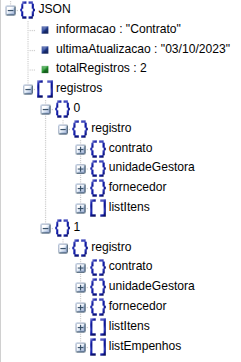
\includegraphics[width=0.4\linewidth]{images/json_contrato_v2.png}
    \caption{Visão em árvore do \glsxtrshort{JSON} de contratos.}
    \label{fig:json-contratos}
\end{figure}

\newpage
No arquivo dos contratos, como mostra a \autoref{fig:json-contratos}, o registro contém as seguintes propriedades:

\subsubsection*{Contrato}
\begin{longtable}{|p{4cm}|p{3cm}|p{2cm}|p{6cm}|}
\hline
\textbf{Nome do Campo} & \textbf{Tipo de Dado} & \textbf{Tamanho} & \textbf{Descrição} \\
\hline
numero & Texto & 20 & Número do contrato. \\
\hline
assinatura & Data & - & Data da assinatura do contrato. \\
\hline
inicioVigencia & Data & - & Data de início da vigência do contrato. \\
\hline
vencimento & Data & - & Data de vencimento do contrato. \\
\hline
valorTotal & Decimal & 10,2 & Valor total do contrato. \\
\hline
objetoResumido & Texto & 255 & Descrição resumida do contrato. \\
\hline
unidadeGestora & Objeto & - & Órgão responsável pelo contrato. \\
\hline
fornecedor & Objeto & - & Fornecedor contratado. \\
\hline
listItens & Objeto & - & Lista de itens do contrato. \\
\hline
listEmpenhos (opcional) & Objeto & - & Lista de empenhos associados ao contrato. \\
\hline
\end{longtable}

\newpage
\subsubsection*{Item do contrato}
\begin{longtable}{|p{4cm}|p{3cm}|p{2cm}|p{6cm}|}
\hline
\textbf{Nome do Campo} & \textbf{Tipo de Dado} & \textbf{Tamanho} & \textbf{Descrição} \\
\hline
numero & Texto & 20 & Número do item. \\
\hline
denominacao & Texto & 100 & Descrição do item. \\
\hline
quantidade & Decimal & - & Quantidade de unidades do item. \\
\hline
unidadeMedida & Texto & 20 & Unidade de medida do item (exemplo: 'Serviço' ou 'Unidade'). \\
\hline
valorUnitario & Texto & 10 & Valor monetário de uma unidade do item. \\
\hline
valorTotal & Texto & 10 & Valor monetário de todas as unidades do item. \\
\hline
\end{longtable}

\subsubsection*{Fornecedor}
\begin{longtable}{|p{4cm}|p{3cm}|p{2cm}|p{6cm}|}
\hline
\textbf{Nome do Campo} & \textbf{Tipo de Dado} & \textbf{Tamanho} & \textbf{Descrição} \\
\hline
pessoa.nome & Texto & 100 & Nome do fornecedor contratado. \\
\hline
\end{longtable}

% ---
% 3 - Capítulo 3
% ---
% ----------------------------------------------------------
\chapter{Trabalhos relacionados}
% ----------------------------------------------------------

A análise de dados abertos governamentais é um tema cada vez mais pertinente na pesquisa acadêmica, especialmente considerando a disponibilidade de algoritmos de aprendizado de máquina e a capacidade de processar grandes quantidades de dados. Nesta seção, são apresentados trabalhos que envolvem a análise de dados de licitações e contratos administrativos e buscam facilitar o combate à corrupção nos processos licitatórios.

A busca bibliográfica foi feita pela plataforma Google Scholar utilizando as palavras-chave "\glsxtrshort{ETL}", "extração transformação e carga", "licitações", "portal de transparência" e "dados abertos". Também foram obtidos trabalhos a partir dos arquivos do Simpósio Brasileiro de Bancos de Dados de 2024 (SBBD).

\cite{schmitz2024sbbd} propõem uma metodologia de aprendizado de máquina que utiliza modelos de mistura gaussiana (GMM) para identificar padrões de lances suspeitos de fraude em processos licitatórios, considerando que a escassez de casos confirmados de fraude torna o uso de métodos de aprendizado supervisionado inviável. O modelo avalia a similaridade entre casos de licitações possivelmente fraudulentas e casos conhecidos de fraude em diversos subespaços, criando um \textit{ranking} eficaz de indicadores de risco.

\cite{schneider2024sbbd} utilizam um conjunto de dados referentes a licitações investigadas pela Operação Lava Jato para avaliar as capacidades de diferentes modelos de aprendizado de máquina em detectar casos de conluio. O trabalho propõe uma metodologia com extração de dados para enriquecimento do conjunto original e técnicas como validação cruzada e otimização de hiperparâmetros para treinar os modelos, alcançando resultados mais precisos.

\cite{santos2021ferramenta} apresentam uma ferramenta para visualizar dados obtidos do Portal de Transparência da Câmara Municipal de Florianópolis; o trabalho foca especificamente nos balancetes de vereadores. Os dados dos documentos em \glsxtrshort{PDF} são extraídos e coletados em arquivos \glsxtrshort{CSV}, que são lidos por uma aplicação escrita na linguagem PHP e adicionados a um banco de dados. Uma interface gráfica permite pesquisar o nome de um vereador e um ano, gerando gráficos dos gastos mensais durante este ano e comparando com gastos de outros anos.

\cite{jesus2021modelo} apresenta um modelo preditivo que utiliza técnicas de mineração de dados e aprendizado de máquina para indicar riscos de irregularidades nas fases de divulgação do edital e apresentação de propostas do processo licitatório. O modelo analisa licitações do Estado de Goiás realizadas entre 2014 e 2019 e calcula o risco utilizando algoritmos de treinamento supervisionado com classificadores. Por fim, constrói-se um \textit{ranking} de licitações potencialmente irregulares.

\cite{mello2024sbbd_estendido} propõem uma modelagem conceitual abrangente de dados para o domínio de licitações, também incluindo dados de fraudes associadas a licitações, denúncias e pessoas envolvidas no processo licitatório, com o objetivo de tornar o projeto de um banco de dados mais robusto e fornecer apoio a sistemas de detecção de fraude. A modelagem inclui uma proposta de persistência poliglota, ou seja, o uso de diversos modelos de banco de dados, como relacional, orientado a grafos e orientado a documentos. 

% <ADICIONAR TABELA COMPARATIVA>
\begin{table}[h]
\caption{Comparação de trabalhos relacionados}
\label{tab:trabalhos-relacionados-1}
\center
\begin{tabular}{| p{0.28\textwidth} | p{0.33\textwidth} | p{0.3\textwidth} |}
\hline
\textbf{Trabalho} & \textbf{Metodologia} & \textbf{Conjunto de dados} \\ \hline
\cite{schmitz2024sbbd} & Aprendizado de máquina com modelos de mistura gaussiana & Licitações referentes à Operação Patrola \\ \hline
\cite{schneider2024sbbd} & \glsxtrshort{ETL} com validação cruzada e otimização de hiperparâmetros & Licitações referentes à Operação Lava Jato \\ \hline
\cite{santos2021ferramenta} & Extração de arquivos \glsxtrshort{CSV} e interface gráfica & Balancetes de vereadores de Florianópolis \\ \hline
\cite{jesus2021modelo} & Mineração de dados e treinamento supervisionado & Licitações do Estado de Goiás entre 2014 e 2019 \\ \hline
\cite{mello2024sbbd_estendido} & Modelagem conceitual com persistência poliglota & - \\ \hline
% \cite{Anvisa2022} & - & - & Sim \\ \hline
% Trabalho proposto & Sim & Não & Sim \\ \hline
\end{tabular}
\fonte{Elaborada pelo autor.}
\end{table}

%\begin{table}[h]
%\caption{Comparação de trabalhos relacionados (parte 2)}
%\label{tab:trabalhos-relacionados-2}
%\center
%\begin{tabular}{| l | c |}
%\hline
%\textbf{Trabalho} & \textbf{Conjunto de dados} \\ \hline
%\cite{schmitz2024sbbd} & Licitações referentes à Operação Patrola \\ \hline
%\cite{schneider2024sbbd} & Licitações referentes à Operação Lava Jato \\ \hline
%\cite{santos2021ferramenta} & Balancetes de vereadores de Florianópolis \\ \hline
%\cite{jesus2021modelo} & Licitações do Estado de Goiás entre 2014 e 2019 \\ \hline
%\cite{mello2024sbbd_estendido} & - \\ \hline
%\end{tabular}
%\fonte{Elaborada pelo autor.}
%\end{table}

% ----------------------------------------------------------
\chapter{Desenvolvimento}
\label{cap:Desenvolvimento}
% ----------------------------------------------------------

Este capítulo descreve o que foi desenvolvido no trabalho de conclusão de curso, incluindo codificação do cliente da \glsxtrshort{API}, análise exploratória de dados coletados, definição do esquema do banco de dados destino implementação do processo de \glsxtrshort{ETL}. 
Todo o código, dados e resultados obtidos neste trabalho estão disponíveis via GitHub\footnote{\url{https://github.com/gustavodesalles/INE5454-trabalho}}.

% ----------------------------------------------------------
\section{Cliente para a \glsxtrshort{API} de compras Públicas da \glsxtrshort{PMF}}
% ----------------------------------------------------------

Ao consultar a \glsxtrshort{API} da prefeitura por meio dos \textit{endpoints} descritos na Seção~\ref{cap:fundamentos}, observou-se que os registros retornados apresentavam informações incompletas. Especificamente, as licitações não possuíam contratos vinculados, e tanto licitações quanto contratos não exibiam os empenhos associados. Este problema indicou que os \textit{endpoints} públicos disponibilizados pela \glsxtrshort{API} forneciam apenas dados resumidos, insuficientes para a análise completa pretendida.

Para contornar essa limitação, foi necessário desenvolver um processo alternativo de extração de dados, baseado nos \textit{endpoints} utilizados internamente pela aplicação Web do portal para alimentar as tabelas de listagem de licitações\footnote{Disponível em: \url{https://transparencia.e-publica.net/epublica-portal/rest/florianopolis/compras/licitacao/listAll}} e contratos\footnote{Disponível em: \url{https://transparencia.e-publica.net/epublica-portal/rest/florianopolis/compras/contrato/listAll}}. Esses \textit{endpoints}, embora não mencionados e descritos na documentação oficial da \glsxtrshort{API}, são responsáveis por fornecer as informações completas que populam dinamicamente as páginas detalhadas de cada licitação ou contrato.

O processo teve início com a execução de uma requisição \glsxtrshort{HTTP} do tipo POST para o \textit{endpoint} que alimenta a tabela de listagem de licitações no portal. O objetivo dessa etapa foi obter os identificadores internos (\textit{IDs}) utilizados pelo sistema para carregar as páginas individuais de cada compra pública. A ferramenta Postman foi empregada tanto para realizar testes nas requisições, como alterar parâmetros de intervalo de tempo e quantidade de registros a serem retornados em uma busca, quanto para capturar os dados e organizá-los em arquivos no formato \glsxtrshort{JSON}, servindo como base para as etapas subsequentes. O mesmo processo foi aplicado ao \textit{endpoint} da tabela de listagem dos contratos.

Na sequência, foi desenvolvido um \textit{script} na linguagem Python, responsável por automatizar o processo de extração. Esse \textit{script} utiliza os \textit{IDs} coletados como parâmetros em requisições POST direcionadas aos \textit{endpoints} responsáveis por retornar os dados completos das licitações\footnote{Disponível em: \url{https://transparencia.e-publica.net/epublica-portal/rest/florianopolis/compras/licitacao/form}} e dos contratos\footnote{Disponível em: \url{https://transparencia.e-publica.net/epublica-portal/rest/florianopolis/compras/contrato/form}}. Os dados extraídos incluem, além das informações da própria licitação, seus contratos vinculados e os respectivos empenhos. Todos os dados obtidos foram armazenados em arquivos \glsxtrshort{JSON} disponibilizados no GitHub\footnote{\url{https://github.com/gustavodesalles/licitacoes-contratos-fln}}.

% ----------------------------------------------------------
\section{Análise exploratória dos dados coletados em \glsxtrshort{JSON}}
% ----------------------------------------------------------

% \attention{Mongo com compass, por exemplo. Cuidado para não deixar redundante com eventuais análises dos dados no BD relacional criado posteriormente. }

Esta etapa visa realizar uma análise exploratória do conjunto de dados obtidos anteriormente com o objetivo de compreender a distribuição dos dados, identificar padrões, avaliar sua consistência e detectar possíveis inconsistências ou lacunas. Para fazer isso, criou-se \textit{scripts} na linguagem Python, utilizando as bibliotecas Pandas e Matplotlib para estruturar os dados e gerar gráficos com base nos atributos dos registros.

Foi analisada a distribuição temporal das datas de assinatura de licitações e contratos ao longo do período abrangido pelos dados coletados. Foram gerados gráficos de séries temporais que representam a quantidade de licitações e contratos registrados por dia. Essa análise permite observar padrões sazonais, concentrações em determinados períodos e eventuais flutuações no volume de registros.

Com o intuito de compreender a composição dos dados, foram geradas distribuições das unidades gestoras vinculadas às licitações presentes no conjunto. Além disso, foi realizada uma análise estatística dos valores estimados das licitações, utilizando gráficos do tipo \textit{boxplot} para identificar a dispersão, a mediana e possíveis valores discrepantes (\textit{outliers}). Esta análise é fundamental para entender a variabilidade dos valores envolvidos nas compras públicas, além de fornecer indícios sobre padrões ou anomalias financeiras.

Outra etapa da análise consistiu na verificação da consistência dos dados financeiros entre os valores das licitações, contratos e respectivos empenhos. Foram comparados os valores dos contratos com os somatórios dos empenhos vinculados, a fim de identificar eventuais divergências e avaliar se os dados refletem corretamente os compromissos financeiros firmados pela administração pública.

Também foi realizada uma análise de integridade e qualidade dos dados, com o levantamento de campos nulos, ausentes ou inconsistentes. Foram identificados registros com ausência de informações relevantes, como dados de fornecedores, valores estimados, datas de assinatura dos contratos ou unidades gestoras. A identificação dessas irregularidades nos dados é fundamental tanto para a correta interpretação dos resultados quanto para o desenvolvimento de eventuais etapas de pré-processamento e limpeza dos dados.

Com os resultados desta análise exploratória, obtém-se uma visão geral do comportamento dos dados e identifica-se limitações a serem consideradas nas etapas subsequentes do trabalho. Além disso, possíveis problemas de completude ou inconsistência nos dados podem indicar falhas nos sistemas de origem ou na própria disponibilização pública das informações.

% ----------------------------------------------------------
\section{Esquema relacional para os dados coletados}
% ----------------------------------------------------------

Nesta seção, é apresentado um esquema de dados modelado com base na \glsxtrshort{API} de compras públicas da \glsxtrlong{PMF} e no dicionário de dados descritos na Seção 2.4. O esquema visa representar a estrutura lógica dos dados de maneira clara e concisa para fins de análise. Um diagrama entidade-relacionamento é apresentado para mostrar a definição das tabelas em formato relacional e suas respectivas conexões.

\begin{figure}[h]
\begin{center}
	\caption{\label{fig:diagrama_er}Diagrama entidade-relacionamento do esquema.}
	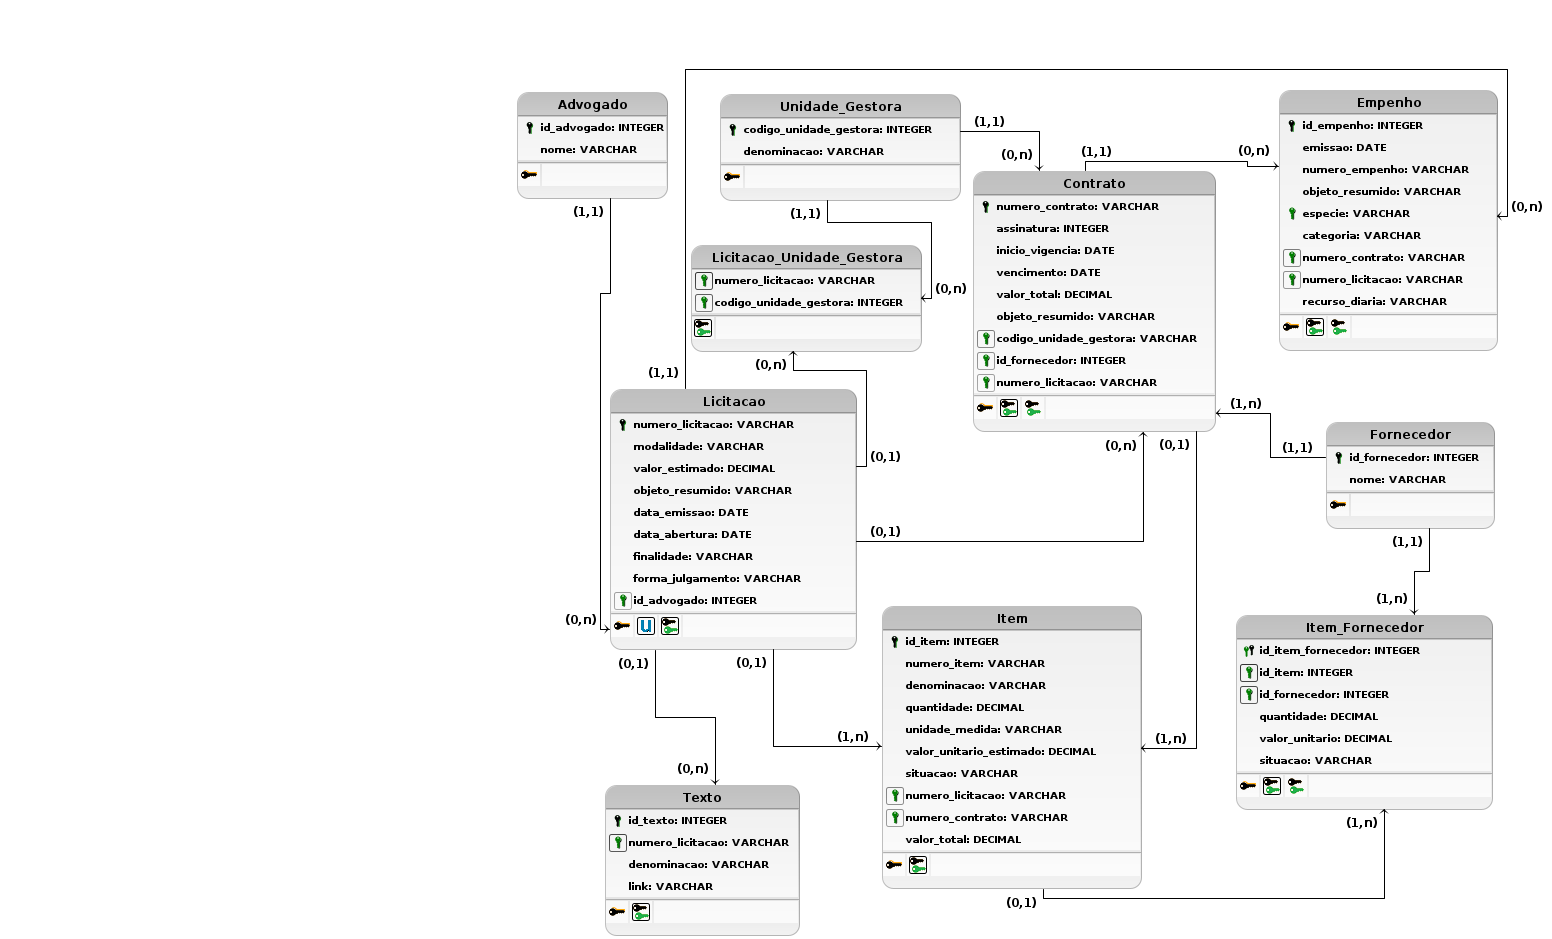
\includegraphics[trim={17cm 0 0 0},clip,width=\textwidth]{images/modelo_logico_tcc_v4.png} %scale=0.32
	\fonte{Elaborada pelo autor.}
\end{center}
\end{figure}

Além das tabelas definidas no dicionário de dados, foi criada uma tabela para representar relações do tipo n:m (muitos-para-muitos); a tabela \texttt{Licitacao\_Unidade\_Gestora} modela a relação entre \texttt{Licitacao} e \texttt{Unidade\_Gestora}, pois uma licitação pode ser vinculada a mais de uma unidade gestora.


% ----------------------------------------------------------
\section{Processo de \glsxtrshort{ETL}}
% ----------------------------------------------------------

Esta seção apresenta o planejamento e implementação do processo de extração, transformação e carga dos dados obtidos nas seções anteriores. As etapas do processo de \glsxtrshort{ETL} serão determinadas após a conclusão da modelagem do esquema relacional dos dados.

% ----------------------------------------------------------
\chapter{Resultados}
\label{cap:Resultados}
% ----------------------------------------------------------

Nesta seção, apresentam-se os resultados obtidos a partir da análise exploratória dos dados de licitações e contratos administrativos da \glsxtrlong{PMF}. O conjunto de dados contempla registros entre 2014 e 2024, abrangendo informações como modalidades de licitação, valores contratados, datas de homologação, prazos de vigência e fornecedores participantes.

A análise exploratória teve como objetivo compreender o comportamento geral dos dados, identificar padrões e tendências ao longo do período, bem como levantar indícios de possíveis irregularidades ou inconsistências cadastrais. Para isso, foram elaborados gráficos e tabelas que sintetizam os aspectos mais relevantes.

Para complementar a análise, a Tabela \ref{tab:modalidades-licitacoes} apresenta um resumo das modalidades de licitações registradas entre 2014 e 2024, considerando o valor total movimentado, a quantidade de processos licitatórios, o número de itens licitados e a quantidade de textos descritivos associados. Observa-se que as modalidades \texttt{Pregão Eletrônico} e \texttt{Dispensa} concentram os maiores valores totais, superando a marca de R\$ 15 bilhões cada. Modalidades tradicionais como \texttt{Pregão Presencial} e \texttt{Concorrência} também apresentam participação relevante, enquanto modalidades menos frequentes, como \texttt{Concurso} e \texttt{Leilão}, apresentam volumes reduzidos. Em particular, nota-se que há 1553 registros de licitações da modalidade \texttt{Pregão}, mas nenhum possui valor monetário, itens ou textos. 

\begin{table}[h]
	\caption{Resumo das modalidades de licitações entre 2014 e 2024}
	\label{tab:modalidades-licitacoes}
	\center
	\begin{tabular}{|l|l|l|l|l|}
		\hline
		\textbf{Modalidade} & \textbf{Valor total (em R\$)} & \textbf{Nº licitações} & \textbf{Nº itens} & \textbf{Nº textos} \\ \hline
		Pregão Presencial & 487201833.11 & 540 & 3688 & 885 \\ \hline
		Inexigibilidade & 228545024.38 & 953 & 609 & 1761 \\ \hline
		Dispensa & 15476798797.17 & 1345 & 2227 & 1598 \\ \hline
		Concorrência & 1199136337.31 & 302 & 271 & 403 \\ \hline
		Pregão & 0 & 1553 & 0 & 0 \\ \hline
		Tomada de Preço & 316345806.41 & 521 & 402 & 313 \\ \hline
		Convite & 6486691903.41 & 87 & 43 & 43 \\ \hline
		Outros & 213741098.32 & 248 & 556 & 161 \\ \hline
		Pregão Eletrônico & 15507026111.65 & 2063 & 31258 & 2831 \\ \hline
		Concurso & 1516107.35 & 1 & 304 & 1 \\ \hline
		Credenciamento & 29404786.46 & 29 & 154 & 64 \\ \hline
		Leilão & 49320025.48 & 3 & 162 & 55 \\ \hline
	\end{tabular}
	\fonte{Elaborada pelo autor.}
\end{table}
% ordenar decrescente valores; números alinhados à direita

A Tabela \ref{tab:modalidades-contratos} relaciona as modalidades de licitações ao número de contratos administrativos formalizados e a quantidade de empenhos vinculados aos processos licitatórios do mesmo período. Devido aos \textit{endpoints} diferentes utilizados para obter os registros dos contratos e empenhos, houve uma quantidade menor de registros retornados em comparação com a consulta da \glsxtrshort{API} pública.

Nota-se a predominância do \texttt{Pregão Eletrônico}, que representa mais de 4 mil contratos e quase 10 mil empenhos, reforçando sua relevância no processo de compras públicas. Modalidades como \texttt{Inexigibilidade} e \texttt{Dispensa} também aparecem com destaque, especialmente no volume de empenhos, sugerindo uso recorrente para aquisições de natureza específica ou emergencial. A modalidade \texttt{Leilão}, apesar de conter somente três licitações, representa 118 contratos, enquanto \texttt{Pregão} e \texttt{Concurso} não possuem nenhum contrato ou empenho.

\begin{table}[h]
	\caption{Resumo das modalidades de contratos entre 2014 e 2024}
	\label{tab:modalidades-contratos}
	\center
	\begin{tabular}{|l|l|l|}
		\hline
		\textbf{Modalidade} & \textbf{Nº contratos} & \textbf{Nº empenhos} \\ \hline
		Pregão Presencial & 396 & 589 \\ \hline
		Inexigibilidade & 492 & 846 \\ \hline
		Dispensa & 797 & 1944 \\ \hline
		Concorrência & 168 & 1949 \\ \hline
		Pregão & 0 & 0 \\ \hline
		Tomada de Preço & 226 & 162 \\ \hline
		Convite & 36 & 0 \\ \hline
		Outros & 378 & 450 \\ \hline
		Pregão Eletrônico & 4220 & 9924 \\ \hline
		Concurso & 0 & 0 \\ \hline
		Credenciamento & 0 & 223 \\ \hline
		Leilão & 118 & 0 \\ \hline
	\end{tabular}
	\fonte{Elaborada pelo autor.}
\end{table}
% colocar valores totais de contratos e empenhos, e números de fornecedores

Esses dados quantitativos fornecem uma visão inicial da distribuição das modalidades ao longo do período analisado, permitindo identificar aquelas que concentram maior movimentação financeira e operacional. Na sequência, são apresentados gráficos que exploram visualmente essas tendências e outros aspectos relevantes das licitações e contratos.

\section*{Distribuição de valores estimados de licitações por unidade gestora}

\begin{figure}[h]
	\begin{center}
		\caption{\label{fig:boxplot_licitacoes}Gráfico \textit{boxplot} de licitações das unidades 1 e 22 no ano de 2024.}
		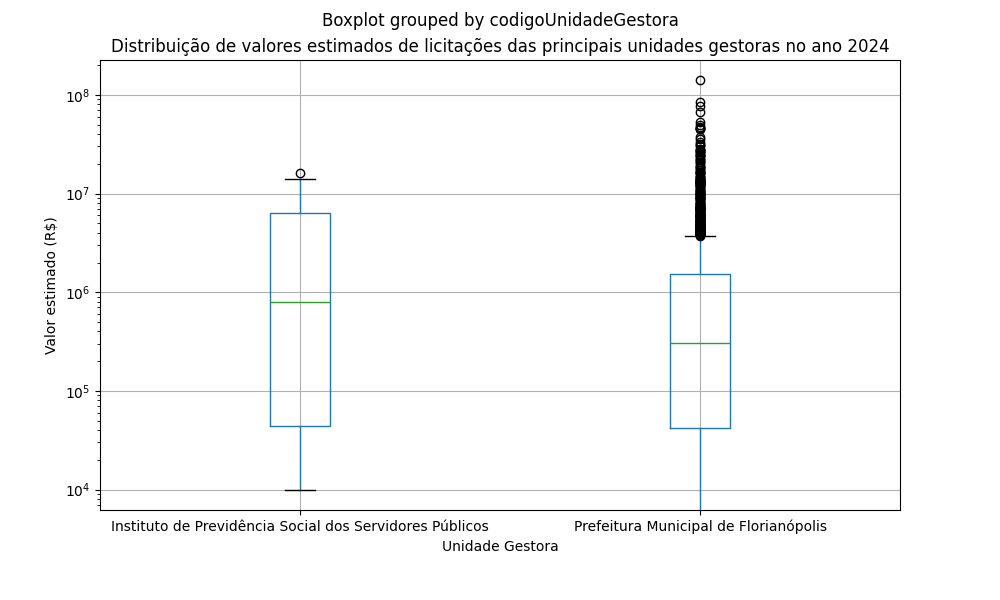
\includegraphics[scale=0.5]{images/boxplot_licitacoes_2024.png} %scale=0.32
		\fonte{Elaborada pelo autor.}
	\end{center}
\end{figure}

%explicar por que foram escolhidas unidades 1 e 22
Em geral, nota-se uma grande quantidade de registros de licitações cuja unidade gestora é a \glsxtrlong{PMF} (código 1) ou o Instituto de Previdência Social dos Servidores Públicos (código 22) que não possuem valores estimados informados. Isto resulta em um \textit{boxplot} com muitos \textit{outliers}, como exemplificado pela \autoref{fig:boxplot_licitacoes}.

Em relação aos contratos, verifica-se uma maior diversidade de unidades gestoras envolvidas, quando comparada às licitações. Essa diferença ocorre mesmo considerando que uma licitação pode estar associada a múltiplas unidades gestoras, enquanto um contrato está vinculado a apenas uma. Além disso, constatou-se uma quantidade significativamente menor de contratos sem o valor total informado, o que denota maior completude dos dados nessa categoria.

Entre todas as licitações analisadas, apenas quatro registros não apresentam unidade gestora informada, sendo todos referentes ao ano de 2024. No caso dos contratos, todos os registros contêm a informação da unidade gestora responsável.

\section*{Quantidade anual de licitações e contratos}

\begin{figure}[h]
	\begin{center}
		\caption{\label{fig:quantidade_licitacoes}Quantidade total de licitações e contratos entre 2014 e 2024.}
		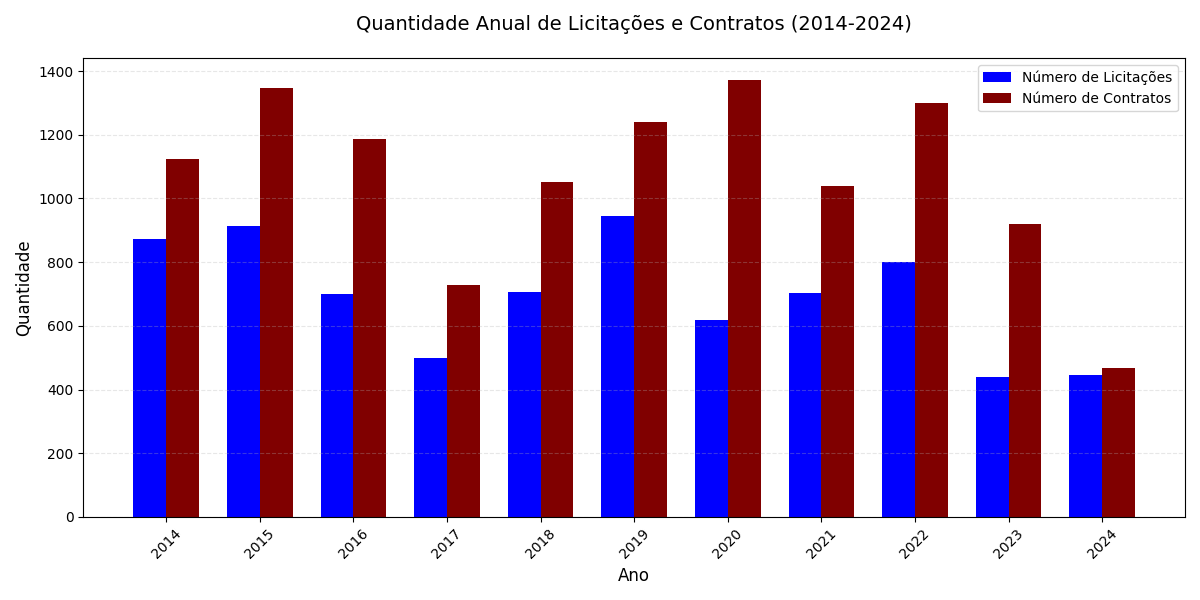
\includegraphics[scale=0.41,trim={0 0 0 2cm},clip]{images/quantidade_anual.png} %scale=0.32
		\fonte{Elaborada pelo autor.}
	\end{center}
\end{figure}

A \autoref{fig:quantidade_licitacoes} compara a quantidade anual de licitações e contratos registrados entre 2014 e 2024. Observa-se que, na maior parte dos anos, o número de contratos supera significativamente o número de licitações, indicando que nem todas as licitações correspondem a um único contrato ou que há contratos decorrentes de processos anteriores.

De 2014 para 2015, há um crescimento tanto nas licitações quanto nos contratos, seguido de quedas expressivas em ambos os indicadores em 2016 e 2017. Considerando o fato de 2016 ter sido um ano de eleição municipal, esta redução está possivelmente relacionada a alterações normativas, restrições orçamentárias ou mudanças nos procedimentos administrativos.

O ano de 2020 apresenta um comportamento atípico: o número de contratos foi mais que o dobro do número de licitações. Isto pode indicar a formalização de múltiplos contratos derivados de um número relativamente reduzido de processos licitatórios, possivelmente como resposta a demandas emergenciais, como as decorrentes da pandemia de COVID-19.

Por fim, o ano de 2024 exibe a menor diferença absoluta entre as quantidades de licitações e contratos em todo o período analisado. Esse alinhamento pode refletir maior proporcionalidade entre a quantidade de processos licitatórios e a execução contratual, sugerindo ajustes na gestão ou no planejamento das aquisições públicas.

Observa-se que houve uma queda do número de registros no ano de 2017 em comparação com os anos anteriores. O ano de 2020 apresenta uma grande discrepância entre os números, sendo a quantidade de contratos maior que o dobro da quantidade de licitações. Em contrapartida, 2024 possui a menor diferença entre licitações e contratos.

\section*{Variação anual de valores totais de licitações e contratos}

\begin{figure}[h]
	\begin{center}
		\caption{\label{fig:variacao_licitacoes}Variação anual de valores totais de licitações e contratos entre 2014 e 2024.}
		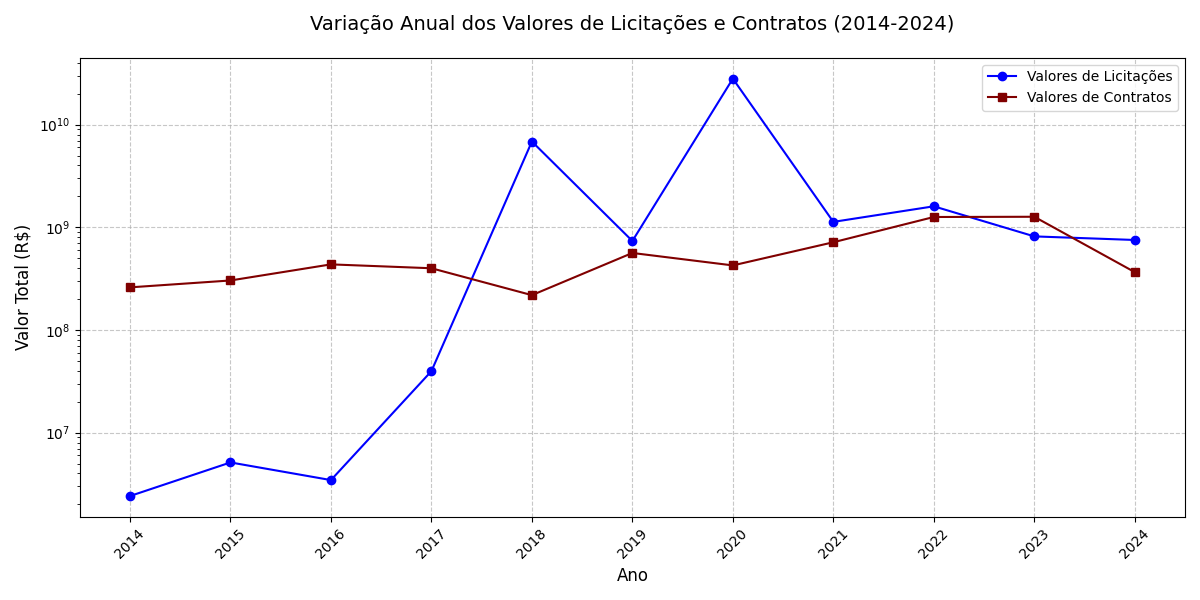
\includegraphics[scale=0.41,trim={0 0 0 2cm},clip]{images/variacao_anual_valores.png} %scale=0.32
		\fonte{Elaborada pelo autor.}
	\end{center}
\end{figure}

A \autoref{fig:variacao_licitacoes} apresenta a variação anual dos valores totais de licitações e contratos registrados entre 2014 e 2024, representados em escala logarítmica para melhor visualização das discrepâncias de ordem de grandeza.

No período inicial, de 2014 a 2017, observa-se que os valores de contratos se mantêm consistentemente superiores aos valores de licitações. Esse comportamento pode ser explicado pelo fato de que muitos contratos são firmados a partir de licitações de anos anteriores ou por contratações diretas, previstas na legislação, que não necessariamente guardam proporcionalidade imediata com os valores licitados no mesmo exercício.

Em 2018, há um crescimento abrupto nos valores de licitações, ultrapassando em larga escala os valores de contratos. Essa discrepância pode estar associada a grandes editais lançados naquele ano, com expressiva previsão orçamentária, mas que não necessariamente se converteram no mesmo volume de contratos firmados de imediato.

Após um aparente equilíbrio no ano de 2019 entre os valores de licitações e contratos, em 2020 observa-se novamente uma disparidade, com os valores licitados alcançando seu ponto mais alto em toda a série, superando em várias ordens de magnitude os valores contratados. Esse comportamento pode estar relacionado a processos emergenciais desencadeados pela pandemia de COVID-19, em que foram anunciados grandes volumes de recursos licitados, mas cuja execução contratual pode ter ocorrido em montantes menores ou em fases posteriores.

A partir de 2021, há uma redução gradual da diferença entre licitações e contratos, atingindo um equilíbrio entre os valores de 2022 em diante. De 2023 até 2024, nota-se uma queda em ambos os índices, ainda que um pouco mais acentuada para os contratos. Essa retração pode refletir tanto um cenário de restrições orçamentárias quanto o processo de adaptação administrativa à plena vigência da nova Lei de Licitações e Contratos (Lei nº 14.133/2021), que se tornou a única lei vigente para licitações e contratações públicas em 2024.

\section*{Principais fornecedores de contratos}

\begin{figure}[h]
	\begin{center}
		\caption{\label{fig:fornecedores}Valores totais gastos com fornecedores de contratos entre 2014 e 2024.}
		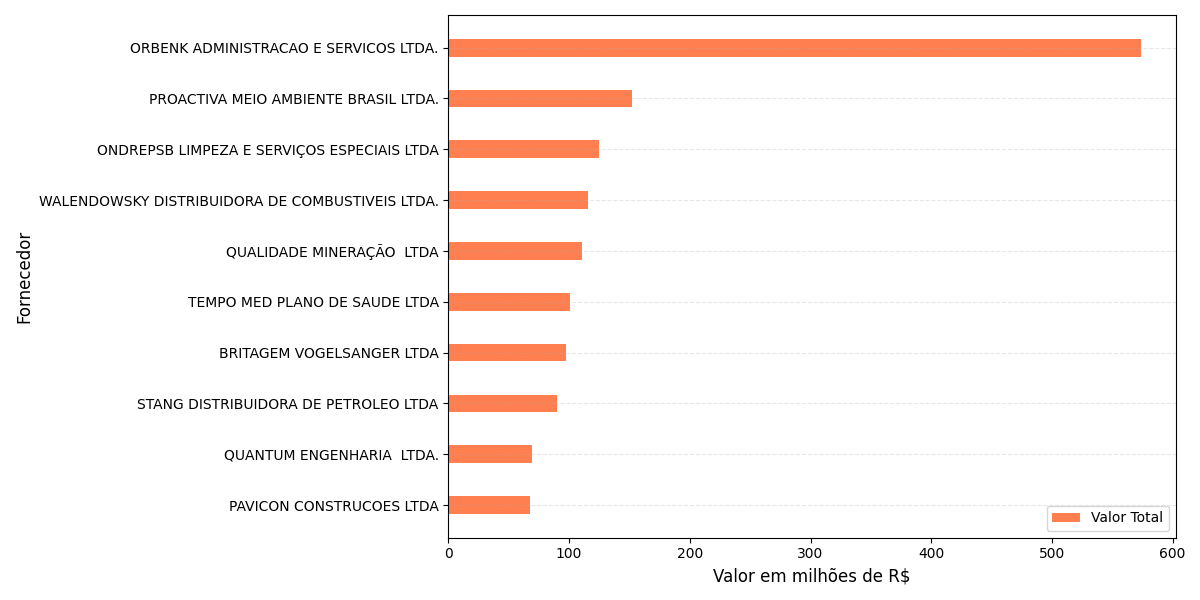
\includegraphics[scale=0.41,clip]{images/principais_fornecedores.png} %scale=0.32
		\fonte{Elaborada pelo autor.}
	\end{center}
\end{figure}

A \ref{fig:fornecedores} apresenta os dez fornecedores com maior valor financeiro total de contratos administrativos firmados com a \glsxtrlong{PMF} durante o período analisado, expressos em milhões de reais.

Nota-se uma forte concentração de recursos em poucos fornecedores. Em particular, o montante da empresa Orbenk Administração e Serviços Ltda. ultrapassa o valor de R\$ 550 milhões, representando uma participação muito superior à das demais. A predominância de empresas como essa e a Ondrepsb Limpeza e Serviços Especiais Ltda. sugere que os serviços de de vigilância patrimonial e limpeza urbana constituem uma parcela significativa das despesas contratuais do município.

Os demais fornecedores listados atuam no setor de obras públicas, como saneamento básico (Proactiva Meio Ambiente Brasil Ltda.), pavimentação de ruas e estradas (Qualidade Mineração Ltda., Britagem Vogelsanger Ltda., Pavicon Construções Ltda.) e iluminação pública (Quantum Engenharia Ltda.), ou na distribuição de combustíveis (Walendowsky Distribuidora de Combustíveis Ltda., Stang Distribuidora de Petróleo Ltda.). A exceção é a empresa Tempo Med Plano de Saúde Ltda., que fornece planos de saúde aos funcionários da Prefeitura.

A análise do gráfico revela, portanto, que a maior parte dos recursos públicos destinados a contratos está concentrada em um número reduzido de fornecedores, com forte destaque para um único ator econômico. Esse cenário pode indicar dependência da administração em relação a determinados prestadores, o que levanta questões importantes sobre concorrência, diversificação de fornecedores e gestão de riscos em contratações públicas.
 

\section*{Comparação entre valores de contratos e empenhos}

\begin{figure}[h]
	\begin{center}
		\caption{\label{fig:contratos_repetidos}Exemplo de múltiplos registros de contratos com números idênticos.}
		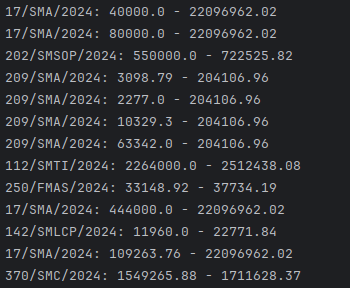
\includegraphics{images/contratos_numeros_repetidos.png} %scale=0.32
		\fonte{Elaborada pelo autor.}
	\end{center}
\end{figure}

% ---
% 4 - Conclusão
% ---
%\phantompart
% ----------------------------------------------------------
\chapter{Conclusões e trabalhos futuros}
\label{cap:Conclusoes}
% ----------------------------------------------------------

As \glsxtrshort{API}s da \glsxtrlong{PMF} oferecem dados incompletos entre si, sendo necessário realizar requisições em diversos \textit{endpoints} para obter informações completas. Para trabalhos futuros, é sugerido o desenvolvimento de uma única \glsxtrshort{API} que reúna todos os conteúdos em um arquivo.

% ----------------------------------------------------------
% ELEMENTOS PÓS-TEXTUAIS
% ----------------------------------------------------------
\postextual
% ----------------------------------------------------------

% ----------------------------------------------------------
% Referências bibliográficas
% ----------------------------------------------------------
\begingroup
    \SingleSpacing\printbibliography[title=REFERÊNCIAS]
\endgroup

% ----------------------------------------------------------
% Glossário
% ----------------------------------------------------------
%
% Consulte o manual da classe abntex2 para orientações sobre o glossário.
%
%\glossary

% ----------------------------------------------------------
% Apêndices
% ----------------------------------------------------------

% ---
% Inicia os apêndices
% ---
%\begin{apendicesenv}
%	\partapendices* 
%	% ----------------------------------------------------------
\chapter{Descrição}
% ----------------------------------------------------------

Textos elaborados pelo autor, a fim de completar a sua argumentação. Deve ser precedido da palavra APÊNDICE, identificada por letras maiúsculas consecutivas, travessão e pelo respectivo título. Utilizam-se letras maiúsculas dobradas quando esgotadas as letras do alfabeto. 

\begin{quadro}[htb]
	\centering
	\caption{\label{qua:Quadro_2}Modelo A.}	
\begin{tabular}{|l|l|}
\hline
xxxx              & yyyyyyyyyyyyyyy    \\
\hline
xxxx              & yyyyyyyyyyyyyyy    \\
\hline
xxxx              & yyyyyyyyyyyyyyy    \\
\hline
xxxx              & yyyyyyyyyyyyyyy    \\
\hline
xxxx              & yyyyyyyyyyyyyyy    \\
\hline
xxxx              & yyyyyyyyyyyyyyy    \\
\hline
xxxx              & yyyyyyyyyyyyyyy    \\
\hline
rrrrrrrrrrrrrrrrr & eeeeeeeeeeeeeeeee  \\
\hline
xxxx              & yyyyyyyyyyyyyyy    \\
\hline
xxxx              & yyyyyyyyyyyyyyy    \\
\hline
rrrrrrrrrrrrrrrrr & eeeeeeeeeeeeeeeee  \\
\hline
xxxx              & yyyyyyyyyyyyyyy    \\
\hline
                  & ttttttttttttttttt  \\
\hline
rrrrrrrrrrrrrrrrr & eeeeeeeeeeeeeeeee  \\
\hline
ttttttttttttt     &                    \\
\hline
rrrrrrrrrrrrrrrrr & eeeeeeeeeeeeeeeee  \\
\hline
rrrrrrrrrrrrrrrrr & eeeeeeeeeeeeeeeee  \\
\hline
                  & gggggggggggggggggg \\
\hline
rrrrrrrrrrrrrrrrr & eeeeeeeeeeeeeeeee  \\
\hline
rrrrrrrrrrrrrrrrr & eeeeeeeeeeeeeeeee  \\
\hline
rrrrrrrrrrrrrrrrr & eeeeeeeeeeeeeeeee  \\
\hline
rrrrrrrrrrrrrrrrr & eeeeeeeeeeeeeeeee  \\
\hline
\end{tabular}
\fonte{Elaborada pelo autor (2016).}
\end{quadro}
%\end{apendicesenv}
% ---


% ----------------------------------------------------------
% Anexos
% ----------------------------------------------------------

% ---
% Inicia os anexos
% ---
%\begin{anexosenv}
%	\partanexos*
%	% ----------------------------------------------------------
\chapter{Descrição}
% ----------------------------------------------------------

São documentos não elaborados pelo autor que servem como fundamentação (mapas, leis, estatutos). Deve ser precedido da palavra ANEXO, identificada por letras maiúsculas consecutivas, travessão e pelo respectivo título. Utilizam-se letras maiúsculas dobradas quando esgotadas as letras do alfabeto. 

%\end{anexosenv}

%---------------------------------------------------------------------
% INDICE REMISSIVO
%---------------------------------------------------------------------
%\phantompart
%\printindex
%---------------------------------------------------------------------

\end{document}
